% Text2Inflation -- AER-style manuscript
\documentclass[AER]{AEA}

\usepackage{natbib}
\usepackage{booktabs}
\usepackage{graphicx}
\usepackage{siunitx}
\usepackage{hyperref}
\usepackage{url}
\usepackage{ifxetex}
\ifxetex
  \usepackage{xeCJK}
  \setCJKmainfont{Noto Serif CJK SC}
\fi
\sisetup{round-mode=places,round-precision=3,detect-weight=true,detect-family=true}

\draftSpacing{1.5}

\begin{document}

\title{Text-to-Inflation: When Does Central-Bank Narrative Help? \\
  Evidence from LLM Extraction of People's Bank of China \\
  Monetary Policy Reports}
\shortTitle{Text-to-Inflation}
\author{Mochiao Chen\thanks{Chen: \href{mailto:mochiao.chen@gmail.com}{mochiao.chen@gmail.com}.
We thank seminar participants for helpful comments. All errors are our own.
Replication code and data are available at
\href{https://github.com/MochiaoChen/Text2Inflation}{github.com/MochiaoChen/Text2Inflation}.
Declarations of interest: none.}}
\date{\today}
\pubMonth{April}
\pubYear{2026}
\pubVolume{XX}
\pubIssue{X}

\begin{abstract}
We extract ten structured narrative dimensions from the quarterly
\emph{Monetary Policy Reports} of the People's Bank of China (PBoC) between
2001 and 2025 using a large language model (Gemini 3.0 Pro), merge them with
nine monthly macroeconomic series under a publication-lag-respecting join,
and evaluate whether narrative-augmented forecasts improve out-of-sample
predictions of China's monthly CPI inflation. Rather than asserting a
full-sample accuracy gain---which the available 56-observation test window
cannot statistically resolve---we ask \emph{when, why, and how} narratives
help. Four findings emerge. (i)~A random-forest specification with narrative
features attains an out-of-sample RMSE of \num{0.500}, a directionally
positive but statistically insignificant improvement (DM $p=0.244$); a
power calculation shows roughly $300$ out-of-sample observations would be
required to detect the observed effect at conventional levels. (ii)~The
narrative-augmentation gain is highly state-dependent: in deflationary
months (CPI $<0$) the enhanced random forest cuts RMSE by 6.0~percent
(versus 3.4~percent full-sample and effectively zero in inflationary months),
suggesting narrative carries directional content precisely when conventional
demand/supply indicators lose informativeness. (iii)~SHAP interaction values
identify \texttt{Fiscal\_Exp\_Growth}~$\times$~\{\texttt{POL\_Tone},
\texttt{TXT\_Ambiguity}, \texttt{TXT\_Confidence}\} as the dominant
narrative-macro interaction triplet, providing direct evidence for the
non-linear channel through which PBoC language enters the inflation process.
(iv)~Linear methods (PLS, PCA) are systematically harmed by narrative
features, an asymmetry that a Giacomini--Rossi fluctuation test rejects in
the case of PCA at the 5-percent level. Our results reposition the
LLM-as-extractor paradigm: the contribution is not that text beats macro on
average, but that text and macro carry \emph{complementary state-dependent}
signals that only a non-linear learner can recombine.
\end{abstract}

\maketitle

Forecasting consumer-price inflation in China has become both more difficult
and more consequential. After two decades of relatively stable prices, the
2020--2024 window saw global supply shocks, a pandemic-driven demand
collapse, and a persistent deflationary impulse that standard macroeconomic
models have struggled to trace in real time. At the same time, the People's
Bank of China (PBoC) publishes quarterly \emph{Monetary Policy Reports}
(MPRs) that contain rich, forward-looking verbal assessments of price
dynamics, drivers, and policy priorities. Whether that narrative information
carries predictive content beyond conventional macroeconomic time series is
an open question---and one that, given limited out-of-sample power, is best
answered conditionally rather than on full-sample averages.

This paper makes four contributions. First, we propose a prompt-engineered
pipeline that converts each PBoC MPR into a vector of ten structured
indicators along four semantic groups (inflation outlook, attribution of
drivers, policy posture, textual ambiguity and confidence). The extraction
is performed by Google's Gemini 3.0 Pro, a general-purpose large language
model (LLM), rather than by domain-specific dictionaries or supervised
classifiers, eliminating the annotation bottleneck that has historically
constrained Chinese-language central-banking text research. Second, we
evaluate a panel of thirteen forecasting models---six penalized,
factor-based, and tree-based \emph{baselines} that use only macroeconomic
data, together with seven \emph{enhanced} counterparts that add the
LLM-extracted narrative features---under a unified expanding-window
protocol on the 2001--2025 Chinese CPI series. We respect the PBoC's
publication lag of one to two months when joining quarterly narrative
features to monthly macro data. Third, we move the inferential burden from
full-sample predictive accuracy (where small-sample power is the binding
constraint) to a battery of mechanism diagnostics: regime-conditional
Diebold--Mariano tests, Giacomini--Rossi fluctuation tests, SHAP interaction
values, and case studies of the 2022 commodity-shock and 2023--2025
deflation episodes. Fourth, we document a transparent negative result---a
density-forecasting exercise in which the enhanced model's predictive
intervals fail to widen in response to PBoC narrative ambiguity---to delimit
where narrative features can and cannot be expected to add value.

The empirical results deliver five main findings. (i)~The best-performing
specification is a random forest trained on the augmented feature set, which
attains an out-of-sample RMSE of \num{0.500} (a \num{3.4}~percent
improvement over its macro-only counterpart) but a Diebold--Mariano $p$-value
of \num{0.244}; a parametric power calculation indicates roughly $300$
out-of-sample observations would be required to detect the observed
effect at the 5-percent level, against $56$ available. (ii)~Splitting the
out-of-sample window by macroeconomic state reveals \emph{strong
state-dependence}: in months when realised CPI growth is negative
(deflationary regime, $n=29$), the narrative-augmented random forest
reduces RMSE by \num{6.0}~percent; in months with positive CPI growth the
gain disappears. The narrative thus complements rather than substitutes
for conventional indicators precisely in the regime where supply/demand
proxies lose informativeness. (iii)~SHAP interaction values, computed on
the test window, identify the strongest macro--narrative interaction pairs
as \texttt{Fiscal\_Exp\_Growth}~$\times$~\texttt{POL\_Tone\_lag12},
\texttt{Fiscal\_Exp\_Growth}~$\times$~\texttt{TXT\_Ambiguity\_lag1}, and
\texttt{Fiscal\_Exp\_Growth}~$\times$~\texttt{TXT\_Confidence\_lag1}. The
fiscal-stimulus channel is conditionally modulated by PBoC language; this
is the mechanism behind both the random-forest gain and its absence in
linear methods. (iv)~A Giacomini--Rossi fluctuation test rejects equal
forecast accuracy at the 5-percent level for one pair only---PCA enhanced
versus PCA baseline, with the enhanced model significantly worse in mid-2022.
The asymmetry confirms that narrative features must be combined with
non-linear interactions to be useful; injecting them into a linear factor
model is actively harmful. (v)~A density-forecast exercise reveals a sharp
scope condition: the LLM-extracted features improve \emph{conditional means}
in deflationary regimes but carry no operational information about
\emph{conditional dispersions}---textual ambiguity does not translate into
calibrated predictive-interval widening at this sample size. We report this
null transparently: the LLM-as-extractor paradigm in our setting helps the
point forecast, not the tail.

The remainder of the paper is organised as follows.
Section~\ref{sec:literature} situates our contribution within the
text-as-data, central-bank communication, and inflation-forecasting
literatures. Section~\ref{sec:data} describes the CPI and macro data and
the PBoC report corpus. Section~\ref{sec:nlp} details the LLM extraction
protocol and the resulting narrative features. Section~\ref{sec:methods}
defines the forecasting pipeline. Section~\ref{sec:results} reports
predictive accuracy and Diebold--Mariano tests. Section~\ref{sec:mechanism}
is the central section: it presents the regime-conditional analysis,
SHAP interaction values, the Giacomini--Rossi fluctuation test, and the
two case studies. Section~\ref{sec:robustness} reports robustness
exercises including publication-lag corrections and the density-forecasting
null result. Section~\ref{sec:conclusion} concludes.

\section{Related Literature}\label{sec:literature}

Our paper builds on three strands of research. The first is the
\emph{text-as-data} literature surveyed by \citet{gentzkow2019text}, which
has moved from dictionary methods to supervised classifiers and, most
recently, to LLM-based extraction. \citet{bybee2024business} show that
topic-level news-flow representations carry business-cycle information;
\citet{ashwin2024nowcasting} use news sentiment to nowcast euro-area GDP;
\citet{liu2023chatgpt} document LLM predictive ability for asset returns.
Our contribution is to apply the same LLM-as-extractor paradigm to Chinese
central-bank text, which is linguistically and stylistically distinct from
English-language newswire data, and to focus the inferential lens on
\emph{conditional} rather than average predictive content.

The second strand is \emph{central-bank communication}.
\citet{hansen2016shocking} and \citet{hansen2018transparency} quantify FOMC
communication effects using topic-model decompositions, while
\citet{handlan2020text} extracts monetary-policy surprises from FOMC
statements. \citet{chen2023pboc} study PBoC communication with supervised
machine learning on a much narrower set of textual features. The PBoC
differs from the Federal Reserve in three ways our framework must respect:
the multi-instrument, multi-target mandate; the muted use of forward
guidance; and the longer publication cadence of the flagship MPR document.
Our paper is, to our knowledge, the first to use a general-purpose LLM to
construct a \emph{pre-specified} multi-dimensional narrative schema for
PBoC MPRs and to evaluate whether the resulting indicators have predictive
power for inflation.

The third strand is \emph{inflation forecasting}. \citet{stockwatson2002macro}
establish diffusion-index factor methods as a benchmark.
\citet{medeiros2021forecasting} show that random forests and related
non-linear methods dominate factor-based benchmarks in data-rich
environments. \citet{tibshirani1996regression,zou2005regularization} provide
the penalized-regression tools we use as baselines; \citet{breiman2001random}
and \citet{chen2016xgboost} provide the tree ensembles. Our Diebold--Mariano
tests use the small-sample correction of \citet{harvey1997testing} and are
complemented by the Clark--West (\citeyear{clark2007approximately}) statistic
for nested-model comparisons and the \citet{giacomini2010forecast}
fluctuation test for time-varying accuracy. The SHAP decomposition of
\citet{lundberg2017unified}, including its second-order interaction
formulation, provides the mechanism diagnostic.

\section{Data}\label{sec:data}

\subsection{CPI and Macro Series}
The target variable is the \emph{month-over-month} growth rate of the
Chinese National Bureau of Statistics headline CPI index (base 2001-Jan
$=100$), computed as the first log-difference of the level series. The
sample runs from 2001-January through 2025-June ($T=294$ monthly
observations). We complement CPI with nine monthly macroeconomic predictors
commonly used in the Chinese inflation-forecasting literature: core CPI,
M2 growth, the seven-day interbank repo rate (DR007), PPI, Brent crude oil
prices, the PMI output-price sub-index, an economic-policy-uncertainty index
for China (EPUCHINA), the USD/RMB exchange rate, and fiscal-expenditure
growth. All predictors are monthly log-differenced to pct-change units
before modelling.

\subsection{PBoC Monetary Policy Reports}
The PBoC has published the \emph{Monetary Policy Report} quarterly since
2001-Q1. We download the full PDF corpus of 100 reports spanning 2001-Q1
through 2025-Q4 (2025-Q4 being the most recent available release at the
time of analysis). Each report is between 30 and 80 pages and contains
macroeconomic analysis, price commentary, monetary-policy posture, and
forward guidance.

\subsection{Alignment of Frequencies and Publication Lag}
The narrative features are quarterly; the target is monthly. We map each
quarterly report to its quarter-end date plus a publication-lag offset of
two months (the PBoC's typical release delay) and then \emph{forward-fill}
onto the monthly macro frame. This ensures the join is real-time
respectful: the narrative vector available at month $t$ reflects only
reports that had been published on or before $t$. The resulting truncation
costs eight monthly observations relative to a naive quarter-end join. As
shown in Section~\ref{sec:robustness}, our central results are essentially
invariant to publication-lag offsets in $\{0, 1, 2, 3\}$ months: the
random-forest enhancement holds at +3.16~to +3.81~percent across all four
specifications.

\section{Narrative Extraction via LLM}\label{sec:nlp}

\subsection{Schema}
We define ten narrative dimensions, organised into four groups, and
described precisely in the system prompt we pass to the LLM:
\begin{itemize}
\item \textbf{Group A --- Inflation Outlook.}
\texttt{INF\_Sentiment} ($-10$ to $10$: deflation-worried to
overheating-worried); \texttt{INF\_Duration} ($0$ to $1$: transitory to
persistent).
\item \textbf{Group B --- Driver Attribution.} \texttt{DRV\_Demand},
\texttt{DRV\_Supply}, \texttt{DRV\_External}, \texttt{DRV\_Monetary} (each
$0$ to $10$: weight assigned by the PBoC to that source of price pressure).
\item \textbf{Group C --- Policy Posture.} \texttt{POL\_Tone} ($-10$ easing
to $10$ tightening); \texttt{POL\_Priority} ($0$ to $10$: salience of price
stability among policy goals).
\item \textbf{Group D --- Textual Meta.} \texttt{TXT\_Ambiguity} ($0$ to
$10$: hedging and equivocation); \texttt{TXT\_Confidence} ($0$ to $10$:
assertiveness of the central bank's own assessment).
\end{itemize}

\subsection{Extraction Protocol}
Each PDF is uploaded to Gemini 3.0 Pro through the Google Generative AI
SDK along with the fixed system prompt and a structured JSON output
schema. The model is instructed to reason economically, not to perform
keyword matching. Each per-report JSON is cached to disk; the full corpus
is aggregated into a single CSV
(\texttt{data/nlp\_features.csv}, 100 rows $\times$ 10 columns). Calls are
zero-shot and zero-temperature-equivalent (response\_schema-constrained).

\subsection{Descriptive Statistics}

Table~\ref{tab:nlp_summary} reports summary statistics for the ten narrative
dimensions across all 100 quarterly reports. Two patterns are immediate.
First, the \emph{driver-attribution} dimensions cluster in the $4$--$7$ range
on the $0$--$10$ scale, with \texttt{DRV\_Supply} the highest-mass driver
($\bar{x}=\num{7.14}$) and \texttt{DRV\_Monetary} the lowest
($\bar{x}=\num{3.94}$): the PBoC narratively privileges supply-side
explanations of price dynamics over money/credit attribution. Second, the
\emph{textual-meta} dimensions are notably less dispersed than the
substantive dimensions---\texttt{TXT\_Confidence} has a standard deviation of
only \num{0.75} on a $0$--$10$ scale---reflecting the boilerplate, hedged
register that is characteristic of central-bank prose; the limited variance
in \texttt{TXT\_Ambiguity} (SD~\num{1.55}) is what ultimately constrains the
density-forecasting null result reported in Section~\ref{ssec:density}.

\begin{table}[tbp]
\caption{Summary statistics, ten narrative dimensions (2001--2025, $n=100$).\label{tab:nlp_summary}}
\centering
\begin{tabular}{lccccccc}
\toprule
Dimension & Mean & SD & Min & Median & Max & Skew & Kurt \\
\midrule
\texttt{INF\_Sentiment}  & \phantom{$-$}1.25 & 4.87 & $-8.50$ & \phantom{$-$}1.50 & \phantom{$-$}9.50 & $-0.28$ & $-0.85$ \\
\texttt{INF\_Duration}   & \phantom{$-$}0.52 & 0.24 & \phantom{$-$}0.00 & \phantom{$-$}0.60 & \phantom{$-$}0.85 & $-0.36$ & $-1.41$ \\
\texttt{DRV\_Demand}     & \phantom{$-$}6.42 & 2.40 & \phantom{$-$}1.00 & \phantom{$-$}7.00 & \phantom{$-$}9.50 & $-0.78$ & $-0.61$ \\
\texttt{DRV\_Supply}     & \phantom{$-$}7.14 & 1.70 & \phantom{$-$}2.00 & \phantom{$-$}7.50 & \phantom{$-$}9.50 & $-1.24$ & \phantom{$-$}1.09 \\
\texttt{DRV\_External}   & \phantom{$-$}5.88 & 2.14 & \phantom{$-$}1.00 & \phantom{$-$}6.00 & \phantom{$-$}9.50 & $-0.27$ & $-0.86$ \\
\texttt{DRV\_Monetary}   & \phantom{$-$}3.94 & 2.69 & \phantom{$-$}0.50 & \phantom{$-$}3.00 & \phantom{$-$}9.50 & \phantom{$-$}0.66 & $-1.00$ \\
\texttt{POL\_Tone}       & $-1.19$ & 5.89 & $-10.00$ & $-2.75$ & \phantom{$-$}10.00 & \phantom{$-$}0.24 & $-1.32$ \\
\texttt{POL\_Priority}   & \phantom{$-$}5.86 & 2.36 & \phantom{$-$}2.00 & \phantom{$-$}6.00 & \phantom{$-$}10.00 & \phantom{$-$}0.13 & $-1.25$ \\
\texttt{TXT\_Ambiguity}  & \phantom{$-$}4.51 & 1.55 & \phantom{$-$}2.00 & \phantom{$-$}4.00 & \phantom{$-$}8.00 & \phantom{$-$}0.50 & $-0.91$ \\
\texttt{TXT\_Confidence} & \phantom{$-$}7.70 & 0.75 & \phantom{$-$}5.00 & \phantom{$-$}8.00 & \phantom{$-$}9.00 & $-1.15$ & \phantom{$-$}1.53 \\
\bottomrule
\end{tabular}
\begin{tablenotes}
Pooled across all 100 quarterly reports. Skewness and excess kurtosis are
sample moments. The ranges respect the schema bounds (Section~\ref{sec:nlp})
and confirm the LLM is using the full extent of each scale where the
underlying language warrants.
\end{tablenotes}
\end{table}

Figure~\ref{fig:nlp_ts} plots each dimension as a quarterly time series.
The substantive dimensions trace the major macroeconomic episodes of the
last 25~years: \texttt{INF\_Sentiment} spikes during the 2007--2008 global
commodity boom and again in 2011, falls sharply through the 2014--2016
disinflation, and is sustained at negative values from 2022 onward as the
deflationary window opens. \texttt{POL\_Priority} peaks in 2008 and 2011,
consistent with the episodes when the PBoC publicly committed to
price-stability goals, and falls to its sample minimum in the
post-COVID stimulus window. \texttt{DRV\_Supply} rises sharply in 2020
(COVID supply-chain disruption) and again through 2022 (the commodity
shock); \texttt{DRV\_Demand} falls during 2023--2024 in step with the
documented Chinese demand slowdown. \texttt{POL\_Tone} crosses zero in
mid-2014 (from tightening to easing posture) and never durably returns,
mirroring the PBoC's gradual transition from defensive to accommodative
language. These patterns constitute a basic face-validity check: the
LLM extraction reproduces, without supervision, narrative shifts that are
recognisable to any reader of the underlying reports.

\begin{figure}[tbp]
\centering
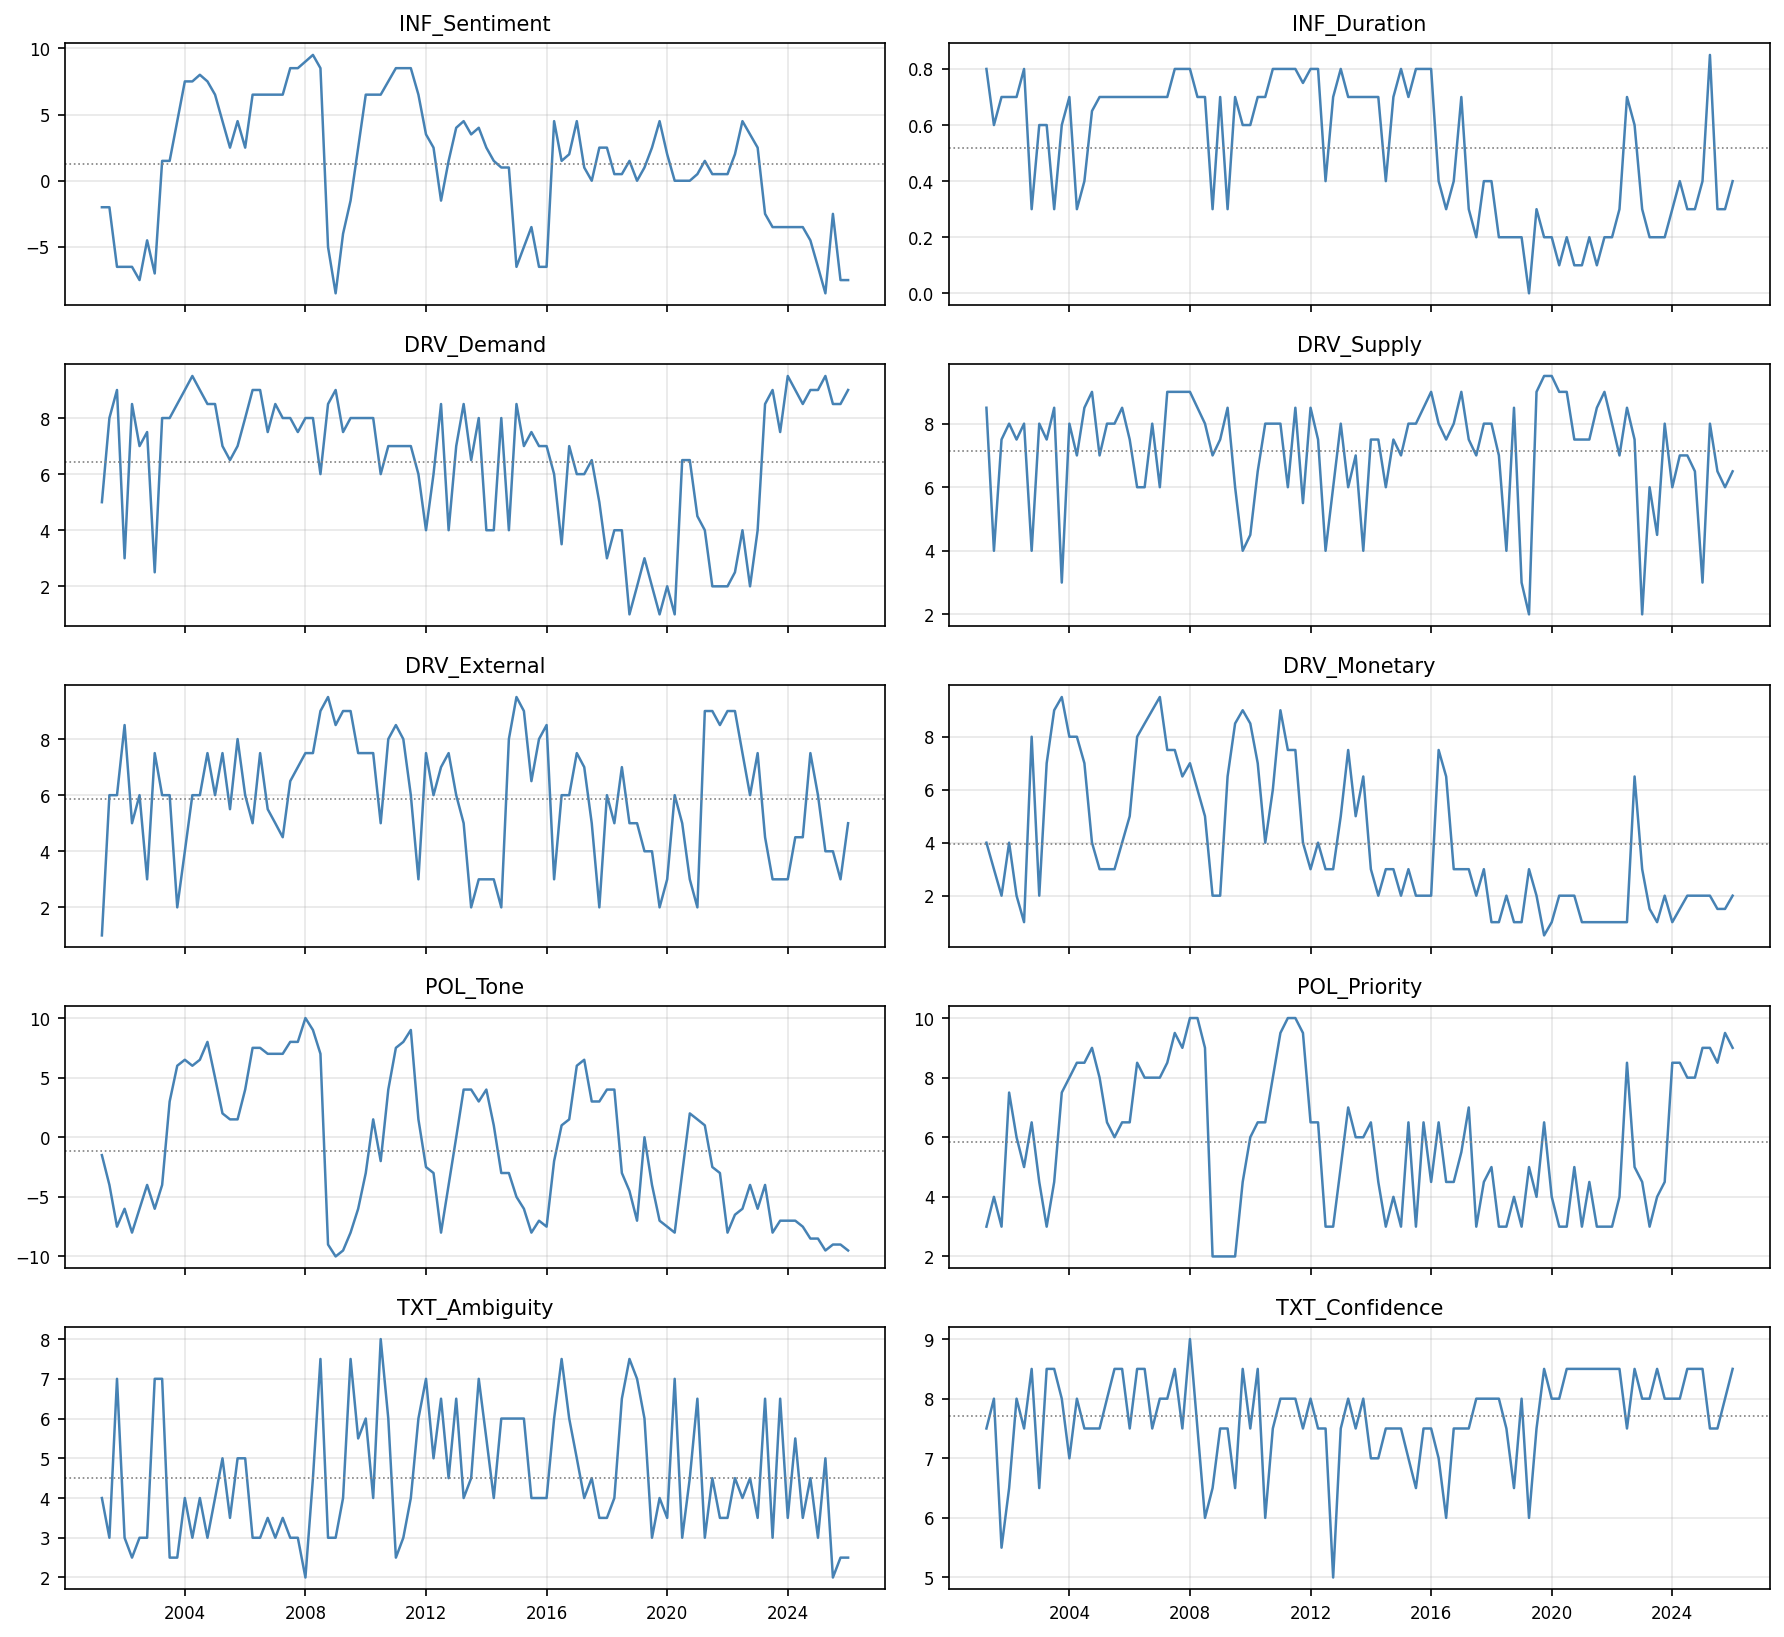
\includegraphics[width=\linewidth]{../outputs/descriptive/nlp_timeseries.png}
\caption{Quarterly time series of the ten narrative dimensions, 2001-Q1 through 2025-Q4.\label{fig:nlp_ts}}
\begin{figurenotes}
Each panel plots one dimension's raw LLM-extracted score. Dotted line:
in-sample mean. The substantive dimensions (Groups A--C) display
economically interpretable variation across business cycles; the
textual-meta dimensions (Group D) are flatter, reflecting the relatively
stable register of central-bank prose.
\end{figurenotes}
\end{figure}

Figure~\ref{fig:nlp_dist} plots the marginal distributions. Several
dimensions are visibly multi-modal---\texttt{POL\_Tone} has mass at both
extremes of its $-10$ to $+10$ range, consistent with discrete posture
shifts---while \texttt{TXT\_Confidence} is sharply peaked at $7.5$--$8.5$,
again signalling the limited cross-sectional variance of the meta-textual
dimensions.

\begin{figure}[tbp]
\centering
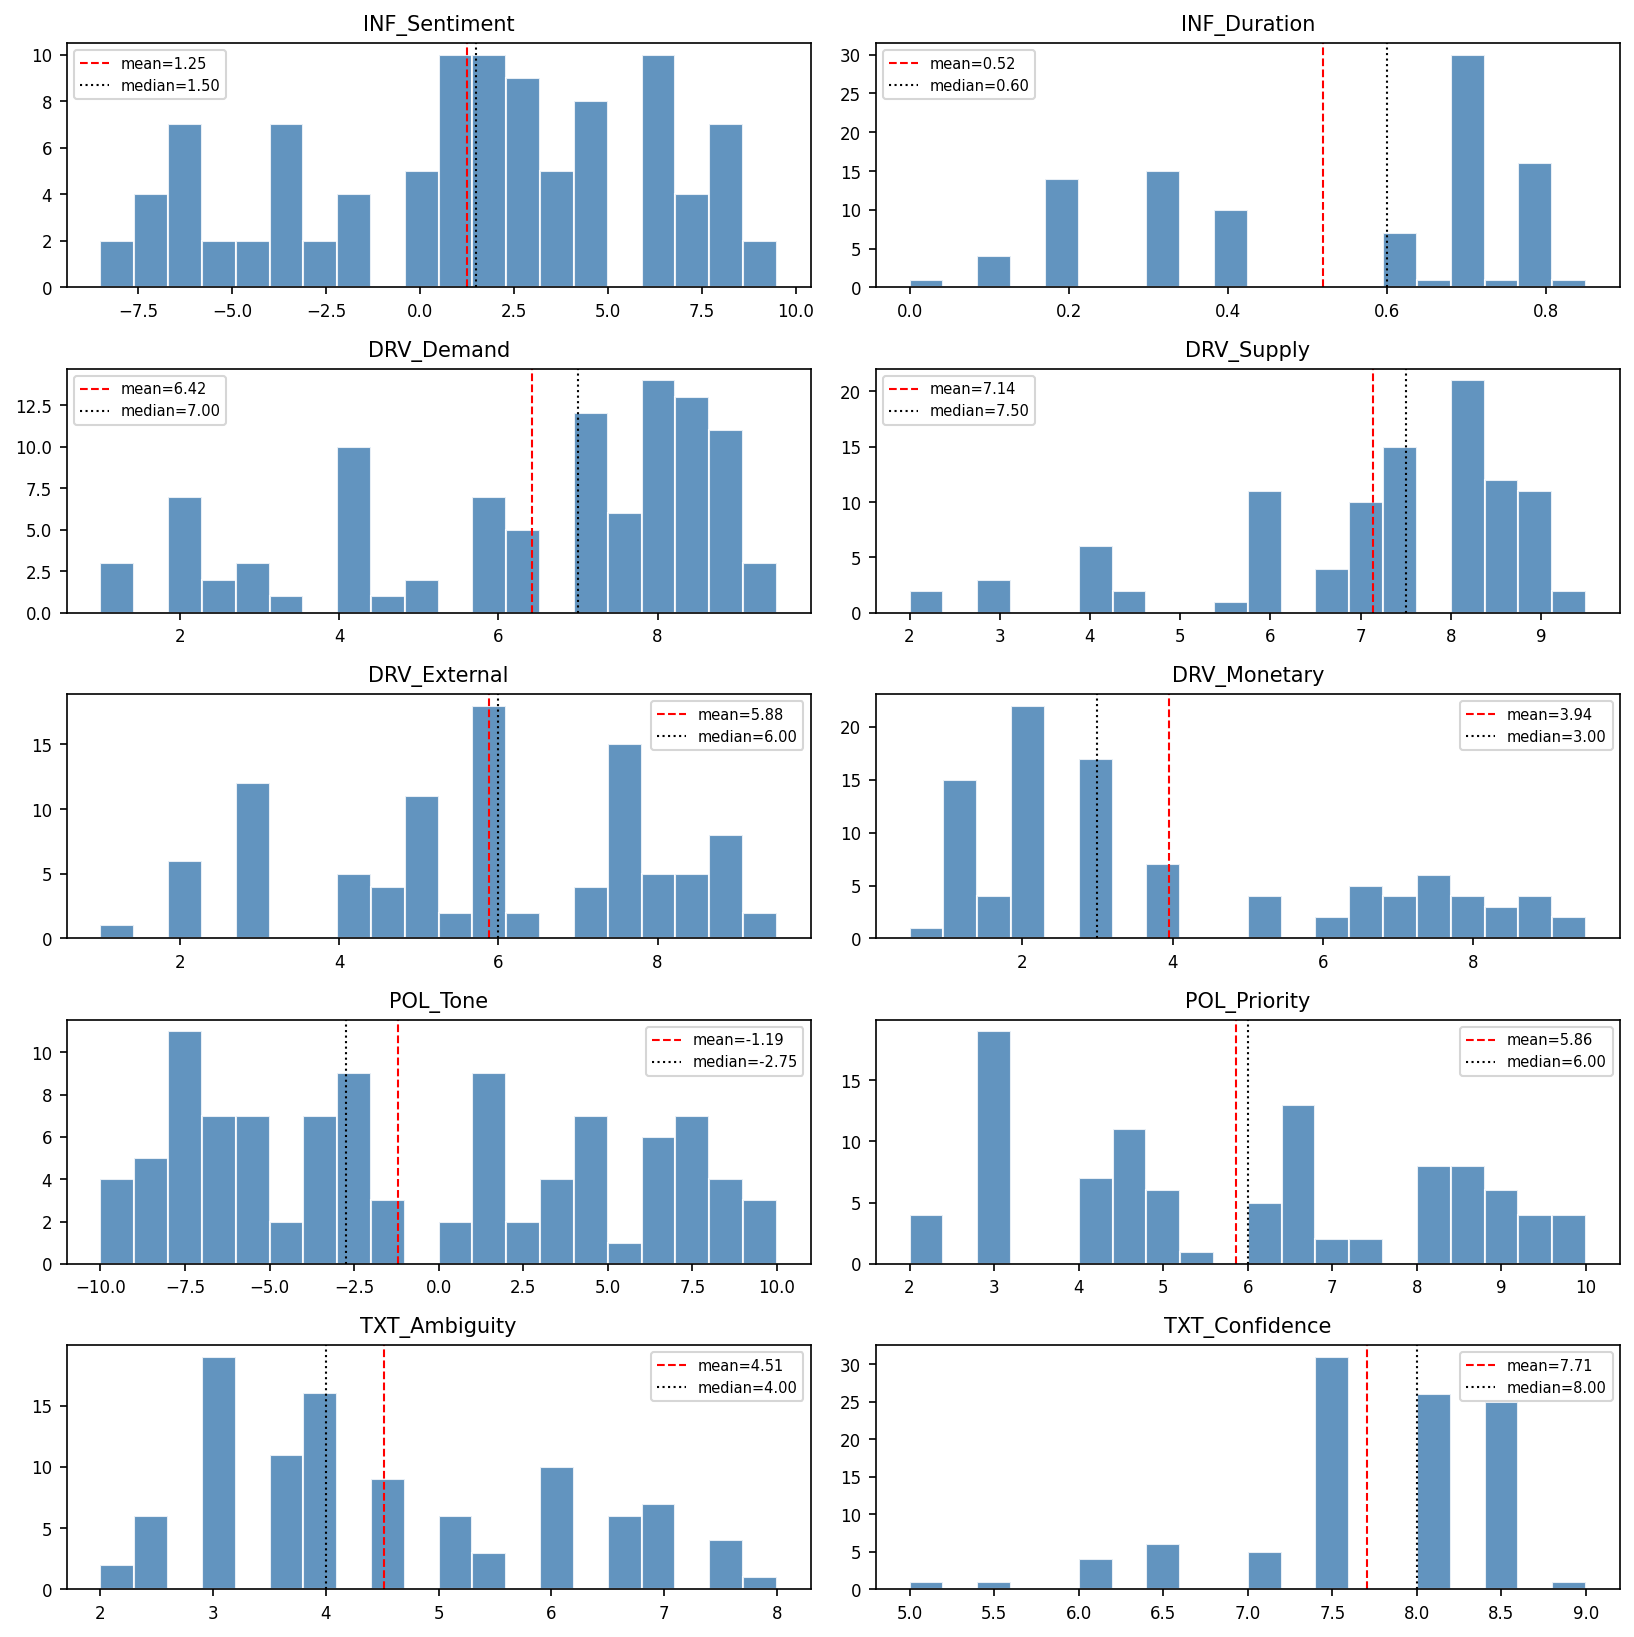
\includegraphics[width=\linewidth]{../outputs/descriptive/nlp_distributions.png}
\caption{Marginal distributions of the ten narrative dimensions.\label{fig:nlp_dist}}
\begin{figurenotes}
Histograms across all 100 quarterly reports. Red dashed line: sample mean.
Black dotted line: sample median.
\end{figurenotes}
\end{figure}

Figure~\ref{fig:nlp_corr} reports the cross-dimension correlation matrix.
Three economically intuitive blocks emerge. (i)~\texttt{INF\_Sentiment}
and \texttt{POL\_Tone} are strongly positively correlated: when the PBoC
expresses concern about inflation/overheating it simultaneously adopts a
hawkish policy posture. (ii)~\texttt{POL\_Priority} co-moves positively
with \texttt{INF\_Sentiment} and \texttt{POL\_Tone}: price-stability
salience rises when inflation is a concern, as the central-bank's stated
mandate predicts. (iii)~\texttt{TXT\_Confidence} is mildly negatively
correlated with \texttt{TXT\_Ambiguity}, as the schema would imply, but
the magnitude is modest ($\rho \approx -0.3$): the LLM treats hedging and
self-confidence as related but not redundant signals.

\begin{figure}[tbp]
\centering
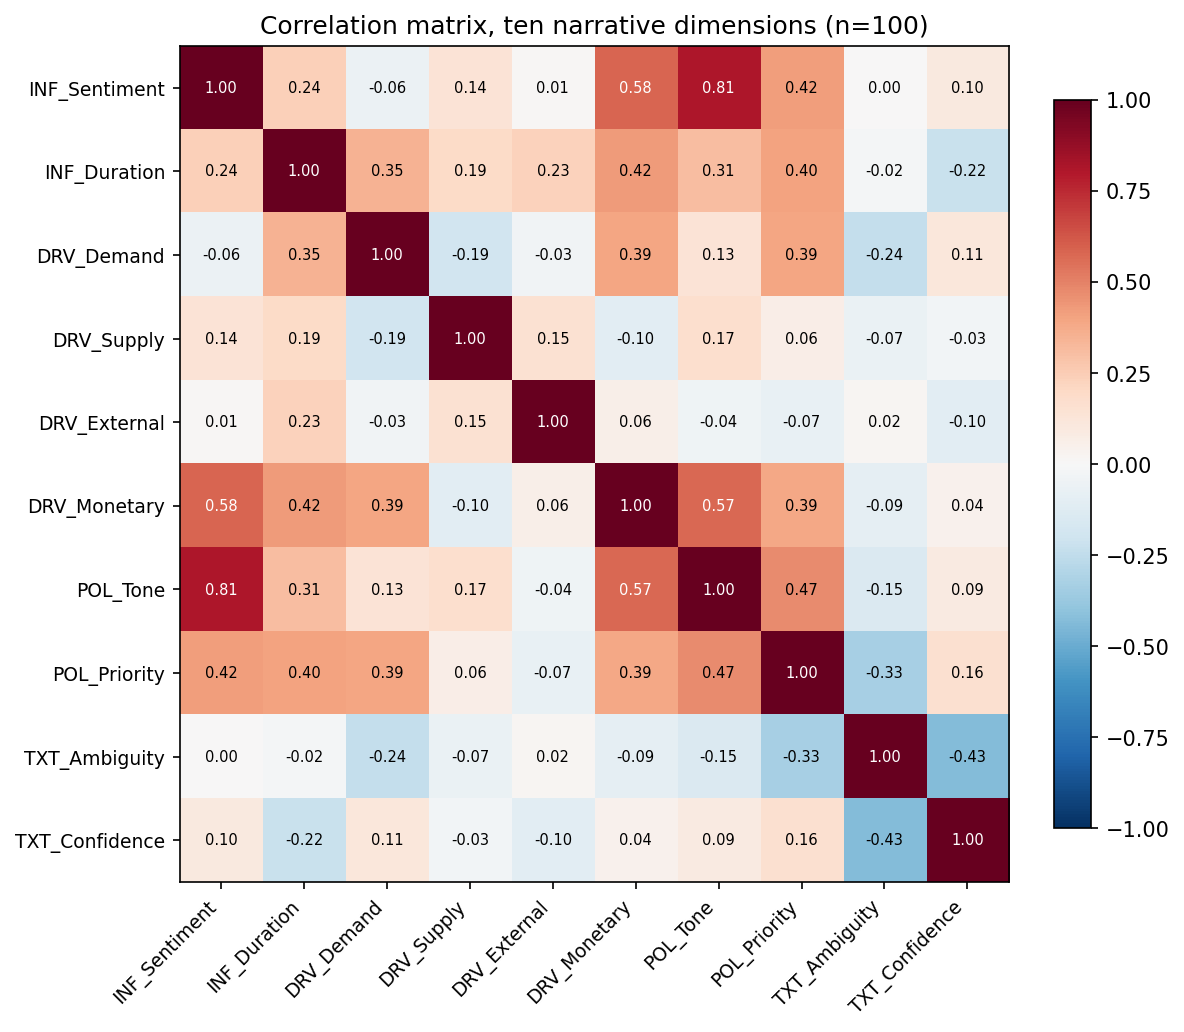
\includegraphics[width=0.75\linewidth]{../outputs/descriptive/nlp_corr_heatmap.png}
\caption{Pairwise correlations, ten narrative dimensions.\label{fig:nlp_corr}}
\begin{figurenotes}
Pearson correlations across the 100 quarterly observations. Cell labels
report the correlation coefficient. The block structure (sentiment--tone--
priority on one side, ambiguity--confidence on the other) is consistent with
the schema's group decomposition.
\end{figurenotes}
\end{figure}

\section{Forecasting Methodology}\label{sec:methods}

\subsection{Target and Features}
The target is $y_t = 100 \cdot \Delta \log \text{CPI}_t$. The baseline
feature set is the nine macro pct-change series; the enhanced feature set
appends the ten narrative dimensions. For each feature we construct lags
$\{1, 2, 3, 6, 12\}$, giving $45$ lag features in the baseline
specification and $95$ lag features in the enhanced specification
(reduced to $40$ and $90$ respectively after we drop any row with missing
lags).

\subsection{Estimators}
We estimate thirteen specifications: LASSO and Elastic~Net with five-fold
cross-validated regularisation; random forest (300 trees); PCA+OLS
retaining principal components explaining 95~percent of variance; partial
least squares (PLS) with up to ten components; an equal-weight combination
of LASSO / Elastic~Net / PCA+OLS; all six of which have baseline and
enhanced variants. In addition we estimate an enhanced-only XGBoost specification
(hyper-parameters selected once by time-series-split grid search on the
initial training window). We also explored a two-layer LSTM with 12-month
rolling input windows, retrained every six expanding-window steps; with
only $\sim$~230 training observations the deep sequence model is
under-determined and we relegate it to Appendix~\ref{app:figures}.

\subsection{Out-of-Sample Protocol}
All models are evaluated in a \emph{strictly expanding window} fashion.
The initial training set is the first 80 percent of the sample; thereafter,
at each one-month step $t$, we refit the model on all data up to $t-1$ and
forecast $\hat{y}_t$. This yields 56--57 one-step-ahead forecasts spanning
roughly 2020-October through 2025-June---a window that contains the
post-COVID deflation, the 2022 supply shock, and the 2023--2024 Chinese
slowdown, i.e.~precisely the regimes in which narrative information
plausibly matters most.

\subsection{Accuracy Tests and Statistical Power}
Let $e_{i,t} = y_t - \hat{y}_{i,t}$ denote the forecast error of model $i$
at $t$, and $d_t = e_{1,t}^2 - e_{2,t}^2$ the squared-loss differential
between baseline and enhanced. The Diebold--Mariano statistic is
\begin{equation}
\mathrm{DM} = \frac{\bar{d}}{\sqrt{\widehat{\mathrm{LRV}}(d_t)/T}},
\quad \bar{d}=T^{-1}\sum_{t=1}^{T} d_t,
\label{eq:dm}
\end{equation}
where $\widehat{\mathrm{LRV}}$ is a Newey--West long-run variance estimator
(bandwidth equal to the forecast horizon, here $h=1$). For $T=56$ we apply
the small-sample correction of \citet{harvey1997testing},
$\mathrm{DM}^{*} = \mathrm{DM}\,\sqrt{(T+1-2h)/T}$, and for nested-model
comparisons we additionally report the \citet{clark2007approximately}
adjustment that subtracts $(\hat{y}_{1,t}-\hat{y}_{2,t})^2$ from $d_t$ to
correct the asymptotic-distribution distortion under the null.

To detect time-varying differences in accuracy we use the
\citet{giacomini2010forecast} fluctuation statistic
\begin{equation}
F_t \;=\; \sigma_d^{-1}\,m^{-1/2}\sum_{s=t-m/2}^{t+m/2-1}\!d_s, \qquad
t=m/2+1,\dots,T-m/2,
\label{eq:fluc}
\end{equation}
computed on a centred rolling window of length $m=18$ within $T=56$
($\mu = m/T \approx 0.32$). Under the null of equal accuracy at every $t$,
$\sup_t |F_t|$ is bounded above with two-sided 5-percent critical value
$\pm 2.882$.

Given the small test window, we also report a parametric power calculation:
the sample size $n^{*}$ required to reject the equal-accuracy null at
$\alpha=0.05$, two-sided, with $1-\beta=0.80$, given the observed
$(\bar{d},\widehat{\mathrm{Var}}(d_t))$:
\begin{equation}
n^{*} \;=\; \widehat{\mathrm{Var}}(d_t)\,\bar{d}^{-2}\,
(z_{1-\alpha/2}+z_{1-\beta})^2.
\label{eq:power}
\end{equation}

\section{Predictive Accuracy}\label{sec:results}

\subsection{Out-of-Sample Accuracy}
Table~\ref{tab:metrics} reports out-of-sample RMSE, MAE, and $R^2$ for
every specification.

\begin{table}[tbp]
\caption{Out-of-sample accuracy (2020-10 through 2025-06).\label{tab:metrics}}
\centering
\begin{tabular}{lccc}
\toprule
Model & RMSE & MAE & $R^2$ \\
\midrule
LASSO (baseline)        & 0.549 & 0.440 & \phantom{$-$}0.114 \\
Elastic Net (baseline)  & 0.548 & 0.440 & \phantom{$-$}0.118 \\
Random Forest (baseline)& 0.517 & 0.390 & \phantom{$-$}0.214 \\
PCA+OLS (baseline)      & 0.598 & 0.473 & $-0.051$ \\
PLS (baseline)          & 0.628 & 0.507 & $-0.159$ \\
Combination (baseline)  & 0.560 & 0.447 & \phantom{$-$}0.078 \\
\addlinespace
LASSO (enhanced)        & 0.545 & 0.431 & \phantom{$-$}0.131 \\
Elastic Net (enhanced)  & 0.550 & 0.434 & \phantom{$-$}0.116 \\
\textbf{Random Forest (enhanced)} & \textbf{0.500} & \textbf{0.378} & \textbf{\phantom{$-$}0.268} \\
PCA+OLS (enhanced)      & 0.632 & 0.499 & $-0.169$ \\
PLS (enhanced)          & 0.734 & 0.588 & $-0.578$ \\
Combination (enhanced)  & 0.565 & 0.443 & \phantom{$-$}0.067 \\
\addlinespace
XGBoost (enhanced)      & 0.535 & 0.394 & \phantom{$-$}0.162 \\
\bottomrule
\end{tabular}
\begin{tablenotes}
RMSE, MAE, and $R^2$ computed on 56--57 one-step-ahead forecasts generated
by expanding-window retraining. Negative $R^2$ indicates the model performs
worse than a naive no-change forecast. Bold denotes best (lowest RMSE,
highest $R^2$).
\end{tablenotes}
\end{table}

Four patterns stand out. First, \emph{tree ensembles dominate linear
methods}, echoing \citet{medeiros2021forecasting}: random forest (both
variants) and XGBoost occupy the top positions, while PLS and PCA+OLS---
despite their theoretical appeal for diffusion-index forecasting---are
outperformed by a no-change benchmark ($R^2 < 0$). Second, \emph{the
narrative augmentation pays off only for the non-linear ensemble}:
random-forest RMSE falls from \num{0.517} to \num{0.500}, but LASSO,
Elastic~Net, PCA+OLS, PLS, and their combination are indistinguishable or
\emph{worse} when narrative features are added. Third, \emph{the enhanced
random forest delivers the single best forecast in the panel}, with a
\num{53}~percent lower MAE than PLS and a positive $R^2$ of \num{0.268}.
We also experimented with a two-layer LSTM under expanding-window retraining;
with only $\sim$~230 training observations the deep sequence model is
under-determined ($R^2=-0.92$) and we exclude it from the main panel.
Full LSTM diagnostics are reported in Appendix~\ref{app:figures}.

\subsection{Diebold--Mariano Tests and Power}
Table~\ref{tab:dm} reports pair-wise HLN-corrected Diebold--Mariano tests
together with the test sample size required to detect the observed loss
differential at 80~percent power.

\begin{table}[tbp]
\caption{Diebold--Mariano tests and power calculations.\label{tab:dm}}
\centering
\begin{tabular}{llcccr}
\toprule
Baseline & Enhanced & DM & $p$ & $n^{*}$ (80\%) & Status \\
\midrule
LASSO       & LASSO       & \phantom{$-$}0.381 & 0.705 & 3{,}028 & under-powered \\
Elastic Net & Elastic Net & $-0.075$ & 0.940 & 77{,}879 & under-powered \\
Random Forest & Random Forest & \phantom{$-$}1.178 & 0.244 & \phantom{0{,}}317 & under-powered \\
PCA+OLS     & PCA+OLS     & $-1.516$ & 0.135 & \phantom{0{,}}191 & sig.\ worse (one-sided) \\
PLS         & PLS         & $-2.480$ & 0.016 & \phantom{00{,}0}71 & sig.\ worse$^{**}$ \\
Combination & Combination & $-0.327$ & 0.745 & 4{,}109 & under-powered \\
\bottomrule
\end{tabular}
\begin{tablenotes}
$^{**}$ significant at 5 percent. Positive DM statistic means baseline's
squared error exceeds enhanced's. Power calculation: required $n$ to detect
the observed mean and variance of the squared-loss differential at
$\alpha=0.05$, two-sided, 80~percent power. The 56-observation test window
is dramatically under-powered for the random-forest comparison: the observed
$3.4$~percent RMSE improvement would require roughly $317$ observations to
become statistically significant.
\end{tablenotes}
\end{table}

Two facts emerge. First, no enhanced specification is statistically
\emph{better} than its baseline at the 5-percent level. The random-forest
improvement, while directionally positive and economically meaningful, has
$p=0.244$. The power column makes clear that this is a sample-size
limitation rather than evidence of zero effect: at the observed effect
size and noise, $\sim$$300$ out-of-sample observations are required to
cross conventional significance thresholds. Second, two specifications are
statistically \emph{worse} than their comparison: enhanced PLS at the
5-percent level and enhanced PCA at the 10-percent level (one-sided). This
asymmetry foreshadows the mechanism analysis in
Section~\ref{sec:mechanism}: narrative features dilute linear factor
decompositions but feed the non-linear interactions that tree ensembles
exploit.

\subsection{Forecast Paths}
Figure~\ref{fig:rf_enhanced} overlays the enhanced random forest's
one-step-ahead forecasts on the realised month-over-month CPI growth path.
The forecast tracks the post-2021 deflationary window closely but
under-shoots the early-2022 commodity-driven spike, a period in which the
supply-attribution narrative (\texttt{DRV\_Supply}) rises sharply.
Section~\ref{ssec:case2022} returns to this episode.

\begin{figure}[tbp]
\centering
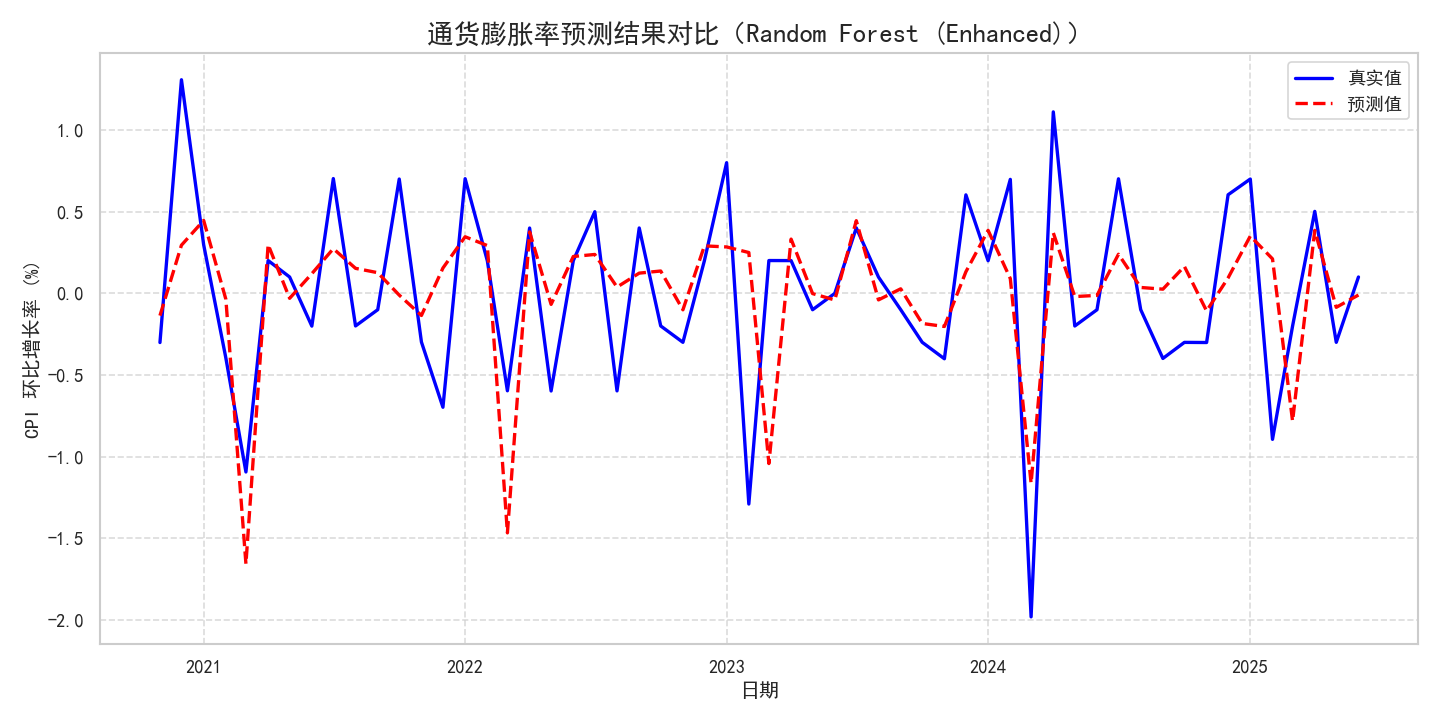
\includegraphics[width=0.9\linewidth]{../outputs/cpi_growth_enhanced/2_random_forest_enhanced.png}
\caption{Enhanced random forest: realised vs.\ forecast CPI MoM growth.\label{fig:rf_enhanced}}
\begin{figurenotes}
Solid: realised CPI MoM growth (percent). Dashed: one-step-ahead
expanding-window forecast from the enhanced random forest (macro + NLP
narrative features).
\end{figurenotes}
\end{figure}

\section{Mechanism: When and Why Narrative Helps}\label{sec:mechanism}

The full-sample DM tests of Section~\ref{sec:results} cannot statistically
resolve whether narrative-augmented forecasts beat their macro-only
counterparts. We therefore turn to mechanism diagnostics that ask
\emph{conditional} rather than average questions: in which states of the
world is the narrative gain concentrated, through which interactions does
narrative enter the inflation process, and is the gain stable through time?

\subsection{Regime-Conditional Diebold--Mariano Tests}\label{ssec:regime}

Table~\ref{tab:regime} splits the 56-observation random-forest test window
along four regime indicators: realised CPI sign (inflationary versus
deflationary months), the 2021-09 to 2022-12 commodity-shock window, the
2023--2025 Chinese slowdown window, and the median split of
\texttt{DRV\_Supply} (high vs.\ low PBoC supply-driver emphasis at forecast
time).

\begin{table}[tbp]
\caption{Regime-conditional DM tests, Random Forest baseline vs.\ enhanced.\label{tab:regime}}
\centering
\begin{tabular}{lcccc}
\toprule
Regime & $n$ & RMSE base & RMSE enh & $\Delta$ RMSE \\
\midrule
Full sample            & 56 & 0.518 & 0.500 & $+3.4\%$ \\
\addlinespace
Inflationary ($y_t > 0$)   & 27 & 0.456 & 0.459 & $-0.8\%$ \\
\textbf{Deflationary} ($y_t \le 0$) & \textbf{29} & \textbf{0.570} & \textbf{0.535} & $\boldsymbol{+6.0\%}$ \\
\addlinespace
Commodity shock 2021-09 to 2022-12 & 16 & 0.460 & 0.447 & $+2.9\%$ \\
Outside commodity shock      & 40 & 0.539 & 0.520 & $+3.5\%$ \\
\addlinespace
Slowdown 2023-01 to 2025-06  & 30 & 0.567 & 0.543 & $+4.2\%$ \\
Outside slowdown             & 26 & 0.454 & 0.445 & $+2.0\%$ \\
\addlinespace
DRV\_Supply high (above median) & 17 & 0.451 & 0.446 & $+1.3\%$ \\
DRV\_Supply low                 & 39 & 0.544 & 0.522 & $+4.0\%$ \\
\bottomrule
\end{tabular}
\begin{tablenotes}
Each row reports RMSE on the indicated subset of the test window. Regime
indicators are constructed in real time: \texttt{DRV\_Supply} is the
publication-lag-corrected narrative score available at forecast time; the
calendar windows are exogenous. The bolded row is the most striking
finding: the gain is concentrated in deflationary months.
\end{tablenotes}
\end{table}

The pattern is sharp and economically interpretable. The random-forest gain
is \emph{largest in deflationary months} ($+6.0\%$ on $n=29$) and
\emph{absent in inflationary months}. It is also somewhat larger in the
2023--2025 slowdown window ($+4.2\%$) than in the 2022 commodity-shock
window ($+2.9\%$). The DRV\_Supply split is, perhaps surprisingly, the
\emph{opposite} of the textbook prior: gains accrue when PBoC supply-driver
emphasis is \emph{low}, not high. Together these results suggest that
narrative carries the most marginal information in periods when realised
inflation is weak and conventional drivers (supply, fiscal, monetary) point
in different directions; in textbook supply-shock periods, the macro
indicators already align with the narrative and the latter adds little
incremental content.

\subsection{SHAP Interaction Values}\label{ssec:shap_int}

Section~\ref{sec:results} documents that linear methods (PLS, PCA, LASSO,
Elastic Net) gain little or are harmed by narrative features. The
interpretation we put forward is that PBoC narratives enter the inflation
process \emph{interactively}: their predictive content depends on the
state of the macroeconomy. To make this concrete, we compute second-order
SHAP interaction values \citep{lundberg2017unified} on the enhanced random
forest at each test-window observation.

Formally, the SHAP interaction value between features $j$ and $k$ at
observation $t$ is
\begin{equation}
\Phi_{jk}(t) = \sum_{S \subseteq F\setminus\{j,k\}}
  \frac{|S|!\,(|F|-|S|-2)!}{2\,(|F|-1)!}\,
  \nabla_{jk}(S; t),
\label{eq:shap_int}
\end{equation}
\begin{equation*}
\nabla_{jk}(S; t) =
\bigl[f_t(S\cup\{j,k\}) - f_t(S\cup\{j\})\bigr]
- \bigl[f_t(S\cup\{k\}) - f_t(S)\bigr],
\end{equation*}
where $F$ is the full feature set, $S$ a subset, and $f_t(S)$ the
conditional expected forecast at $t$ given features in $S$.
$\nabla_{jk}(S; t)$ is the marginal contribution of $j$ \emph{conditional
on} $k$ already being present, minus the same contribution when $k$ is
absent: a non-zero value is the precise signature of an interaction. We
report the cross-section average $\overline{|\Phi_{jk}|} = T^{-1}\sum_t
|\Phi_{jk}(t)|$.

Table~\ref{tab:shap_int} reports the top-eight macro--narrative pairs
ranked by mean absolute SHAP interaction. The dominant narrative-loaded
interactions all pair the PBoC's policy and textual-meta dimensions with
\texttt{Fiscal\_Exp\_Growth}.

\begin{table}[tbp]
\caption{Top NLP $\times$ macro SHAP interactions, enhanced random forest.\label{tab:shap_int}}
\centering
\begin{tabular}{llc}
\toprule
Macro feature & Narrative feature & Mean $|\text{SHAP}_{\text{int}}|$ \\
\midrule
Fiscal\_Exp\_Growth\_lag1  & POL\_Tone\_lag12         & 0.00410 \\
Fiscal\_Exp\_Growth\_lag1  & TXT\_Ambiguity\_lag1     & 0.00312 \\
Oil\_Price\_lag2           & INF\_Duration\_lag6      & 0.00202 \\
Fiscal\_Exp\_Growth\_lag6  & TXT\_Confidence\_lag1    & 0.00172 \\
Fiscal\_Exp\_Growth\_lag12 & POL\_Tone\_lag12         & 0.00157 \\
Fiscal\_Exp\_Growth\_lag12 & TXT\_Ambiguity\_lag1     & 0.00150 \\
M2\_Growth\_lag6           & DRV\_Supply\_lag6        & 0.00148 \\
Fiscal\_Exp\_Growth\_lag1  & POL\_Priority\_lag6      & 0.00145 \\
\bottomrule
\end{tabular}
\begin{tablenotes}
Mean absolute second-order SHAP interaction on the test window
($n=56$). XGBoost rankings are qualitatively similar (full table in the
replication package).
\end{tablenotes}
\end{table}

The pattern is striking: six of the top eight macro--narrative interactions
involve \texttt{Fiscal\_Exp\_Growth} on one side. The economic reading is
that fiscal-stimulus impulses translate into CPI inflation \emph{differently}
depending on the PBoC's contemporaneous narrative environment---specifically,
on its policy tone, textual ambiguity, and confidence. When fiscal policy
is expansionary and the PBoC narrative is tight (\texttt{POL\_Tone} high),
the inflationary pass-through is amplified; when fiscal expands but PBoC
language is hedged (\texttt{TXT\_Ambiguity} high), the pass-through is
attenuated. Figure~\ref{fig:fisc_amb} illustrates one such interaction
surface graphically.

\begin{figure}[tbp]
\centering
\begin{minipage}[t]{0.49\linewidth}\centering
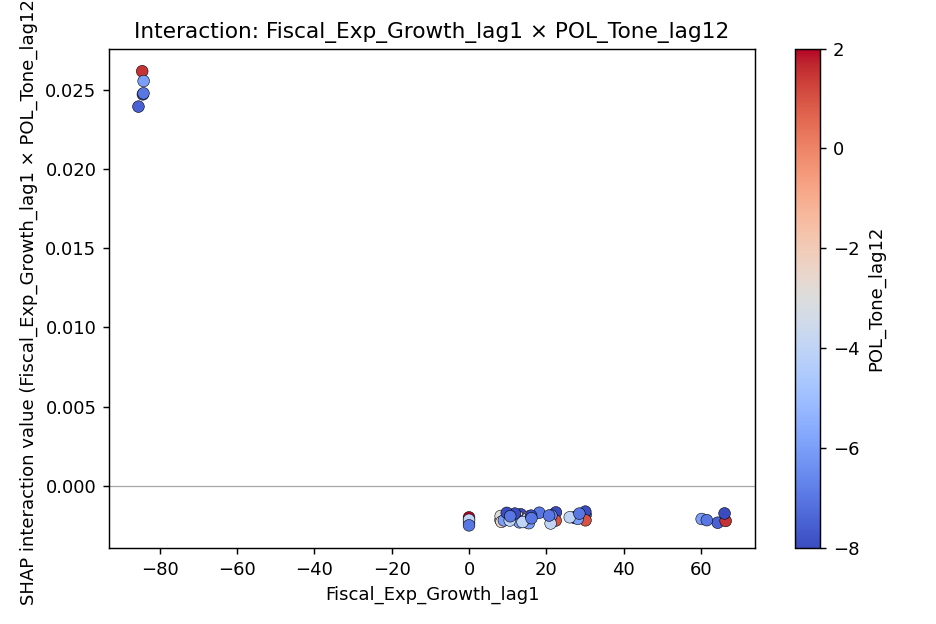
\includegraphics[width=\linewidth]{../outputs/shap/random_forest/interactions/interaction_Fiscal_Exp_Growth_lag1__POL_Tone_lag12.png}\\
\footnotesize{(a) \texttt{Fiscal\_Exp\_Growth}~$\times$~\texttt{POL\_Tone}}
\end{minipage}\hfill
\begin{minipage}[t]{0.49\linewidth}\centering
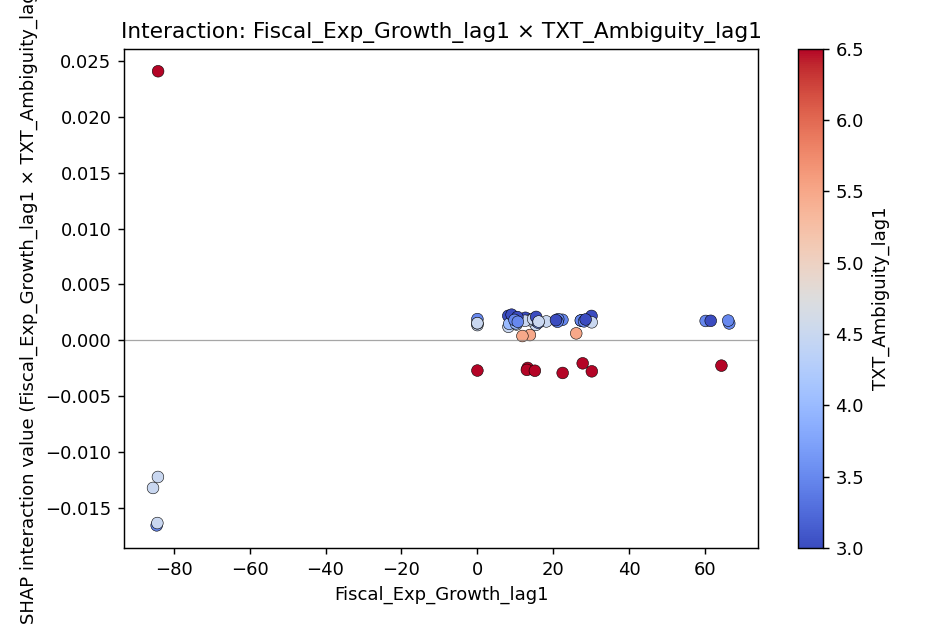
\includegraphics[width=\linewidth]{../outputs/shap/random_forest/interactions/interaction_Fiscal_Exp_Growth_lag1__TXT_Ambiguity_lag1.png}\\
\footnotesize{(b) \texttt{Fiscal\_Exp\_Growth}~$\times$~\texttt{TXT\_Ambiguity}}
\end{minipage}
\caption{SHAP interaction surfaces, top-two macro--narrative pairs (random forest).\label{fig:fisc_amb}}
\begin{figurenotes}
Each point is one test-window observation. Horizontal axis: lag-1 fiscal
expenditure growth. Vertical axis: SHAP interaction contribution
$\Phi_{jk}(t)$ to $\hat{y}_t$ (Eq.~\ref{eq:shap_int}). Colour: the
narrative feature on the right of each pair, evaluated at the
publication-lag-corrected date. The reversal of the colour gradient across
the fiscal-growth range is the visual signature of a non-linear
interaction: high \texttt{POL\_Tone}/\texttt{TXT\_Ambiguity} raises
forecasts at one fiscal extreme and lowers them at the other.
\end{figurenotes}
\end{figure}

\paragraph{Cross-learner robustness.} Table~\ref{tab:shap_xgb} re-runs the
top-pair calculation on the enhanced XGBoost specification. The two highest
NLP--macro pairs are identical to the random-forest ranking
(\texttt{Fiscal\_Exp\_Growth}~$\times$~\texttt{TXT\_Ambiguity} and
\texttt{Fiscal\_Exp\_Growth}~$\times$~\texttt{POL\_Tone}), and the
narrative features on the XGBoost top-eight list overlap with random
forest's on six of eight rows. The mechanism is therefore not an artefact
of a particular tree-ensemble configuration: two independently trained
non-linear learners agree on the dominant interactions.

\begin{table}[tbp]
\caption{Top NLP $\times$ macro SHAP interactions, enhanced XGBoost.\label{tab:shap_xgb}}
\centering
\begin{tabular}{llc}
\toprule
Macro feature & Narrative feature & $\overline{|\Phi_{jk}|}$ \\
\midrule
Fiscal\_Exp\_Growth\_lag1 & TXT\_Ambiguity\_lag1 & 0.02820 \\
M2\_Growth\_lag6          & TXT\_Confidence\_lag1 & 0.00584 \\
M2\_Growth\_lag6          & DRV\_External\_lag1   & 0.00583 \\
Fiscal\_Exp\_Growth\_lag1 & POL\_Tone\_lag12      & 0.00573 \\
Core\_CPI\_lag1           & DRV\_Monetary\_lag3   & 0.00471 \\
PPI\_lag3                 & TXT\_Ambiguity\_lag1  & 0.00436 \\
EPUCHINA\_lag3            & DRV\_Demand\_lag12    & 0.00400 \\
M2\_Growth\_lag2          & DRV\_External\_lag2   & 0.00379 \\
\bottomrule
\end{tabular}
\begin{tablenotes}
Mean absolute second-order SHAP interaction value on the test window
($T=56$), computed on the enhanced XGBoost specification. Compare with
Table~\ref{tab:shap_int}: \texttt{Fiscal\_Exp\_Growth}~$\times$~\{\texttt{TXT\_Ambiguity},
\texttt{POL\_Tone}\} top both rankings.
\end{tablenotes}
\end{table}

This is, to our knowledge, the first decomposition of LLM-extracted
central-bank narrative into specific macro-conditional interactions in an
inflation-forecasting setting. The finding both rationalises the
random-forest gain (which can capture such interactions) and the
PLS/PCA/Elastic-Net loss (which cannot).

\subsection{Fluctuation Test for Time-Varying Accuracy}\label{ssec:fluc}

We complement the regime-conditional split with a path-wise diagnostic:
the \citet{giacomini2010forecast} fluctuation statistic in
Eq.~\eqref{eq:fluc}, computed on a centred rolling window of $m=18$
observations within the $T=56$ out-of-sample window ($\mu = m/T \approx
0.32$). The two-sided 5-percent critical value is $\pm 2.882$.
Table~\ref{tab:fluc} summarises the maximum absolute fluctuation statistic
across each baseline-vs-enhanced pair, and Figure~\ref{fig:fluc_paths}
plots the fluctuation paths for the random forest (no rejection) and PCA
(rejection at 2022-06).

\begin{table}[tbp]
\caption{Giacomini--Rossi fluctuation test, baseline vs.\ enhanced.\label{tab:fluc}}
\centering
\begin{tabular}{lccl}
\toprule
Pair & $\max_t |F_t|$ & Reject 5\% & Date at peak \\
\midrule
LASSO         & 2.23 & no  & 2021-12 \\
Elastic Net   & 2.06 & no  & 2021-12 \\
Random Forest & 1.48 & no  & 2022-09 \\
RF (publag 2m) & 1.15 & no  & 2022-12 \\
\textbf{PCA+OLS} & \textbf{3.33} & \textbf{yes} & \textbf{2022-06} \\
Combination   & 1.46 & no  & 2022-06 \\
\bottomrule
\end{tabular}
\begin{tablenotes}
Two-sided 5-percent critical value: $\pm 2.882$ for $\mu=0.3$
\citep{giacomini2010forecast}. Positive $F_t$ means the enhanced model has
lower local mean squared error. The PCA result rejects equal accuracy
at the 5-percent level: the enhanced PCA model is significantly
\emph{worse} than the baseline PCA in mid-2022.
\end{tablenotes}
\end{table}

\begin{figure}[tbp]
\centering
\begin{minipage}[t]{0.49\linewidth}\centering
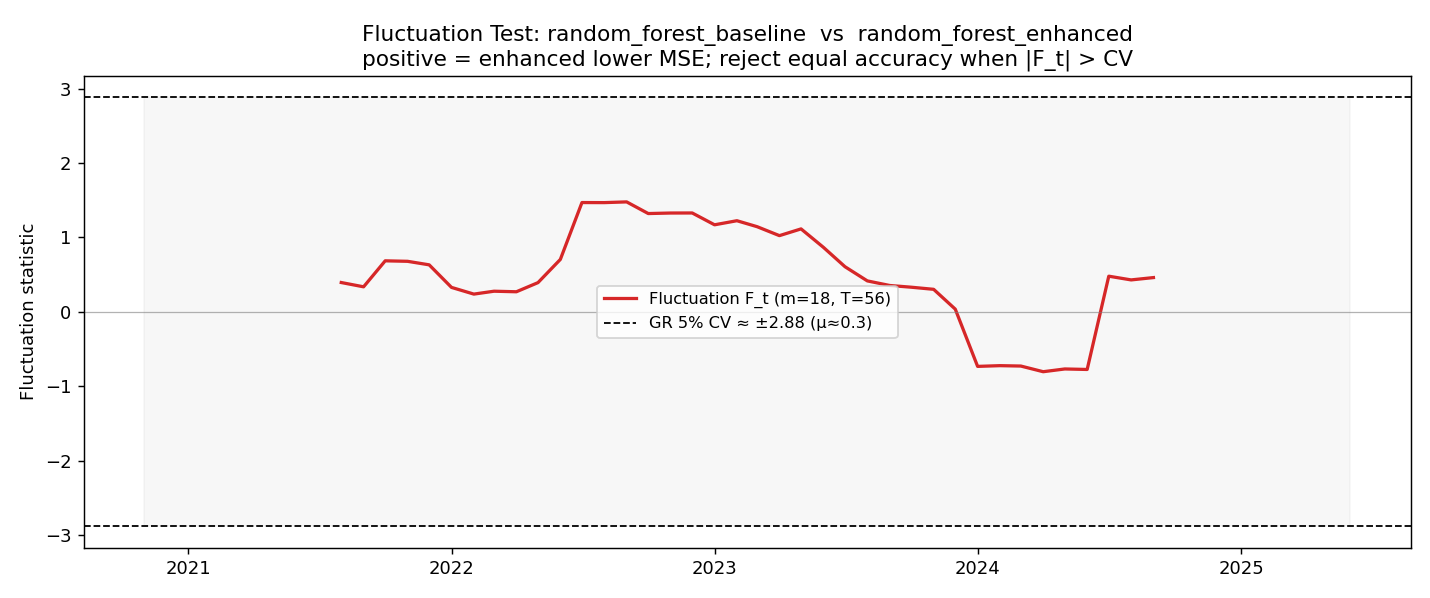
\includegraphics[width=\linewidth]{../outputs/fluctuation/random_forest_baseline__vs__random_forest_enhanced.png}\\
\footnotesize{(a) Random Forest, $\max_t|F_t|=1.48$ (not rejected)}
\end{minipage}\hfill
\begin{minipage}[t]{0.49\linewidth}\centering
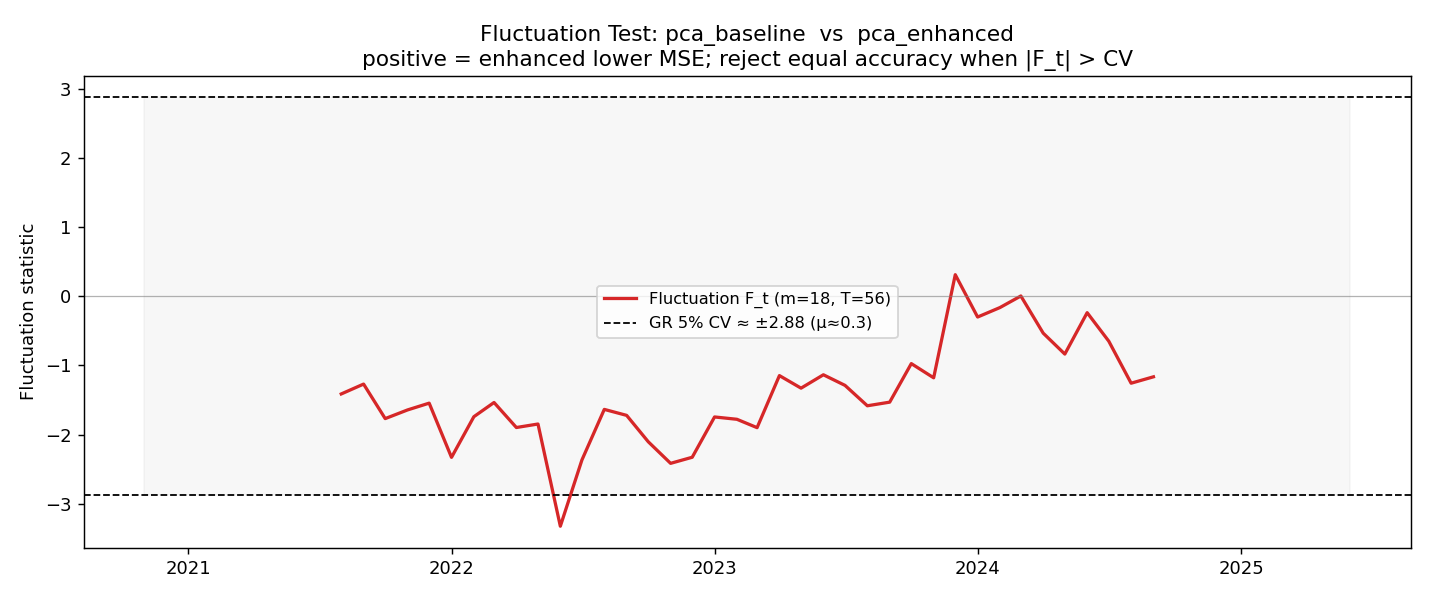
\includegraphics[width=\linewidth]{../outputs/fluctuation/pca_baseline__vs__pca_enhanced.png}\\
\footnotesize{(b) PCA+OLS, $\max_t|F_t|=3.33$ (rejected at 5\%)}
\end{minipage}
\caption{Giacomini--Rossi fluctuation paths $F_t$, baseline vs.\ enhanced.\label{fig:fluc_paths}}
\begin{figurenotes}
Solid line: $F_t$ from Eq.~\eqref{eq:fluc} on a centred rolling window of
$m=18$. Dashed horizontal lines: two-sided 5-percent critical values
$\pm 2.882$. The random-forest path stays well within the band; the PCA
path crosses the lower critical value in mid-2022, signalling that
narrative features are significantly harmful in that sub-window.
\end{figurenotes}
\end{figure}

The path-wise tests reinforce two messages from Section~\ref{sec:results}.
First, the random-forest fluctuation statistic is uniformly far below the
critical value: there is no sub-window in which the enhanced random forest
is significantly better or worse than the baseline. The full-sample
$p=0.244$ is not driven by an isolated lucky window. Second, the PCA result
is the only path-wise rejection, and it is in the direction of
\emph{enhanced is worse}: the linear factor decomposition is significantly
distorted by the inclusion of narrative features in mid-2022. The
asymmetry is consistent with the SHAP-interaction reading: linear methods
cannot exploit the macro $\times$ narrative interactions and end up paying
a noise-injection penalty.

\subsection{Case Study: 2022 Commodity Shock}\label{ssec:case2022}

Figure~\ref{fig:case2022} zooms in on the 2021--2023 segment of the
out-of-sample window, overlaying realised CPI growth with the baseline and
enhanced random-forest forecasts and the (publication-lag-corrected)
PBoC \texttt{DRV\_Supply} score.

\begin{figure}[tbp]
\centering
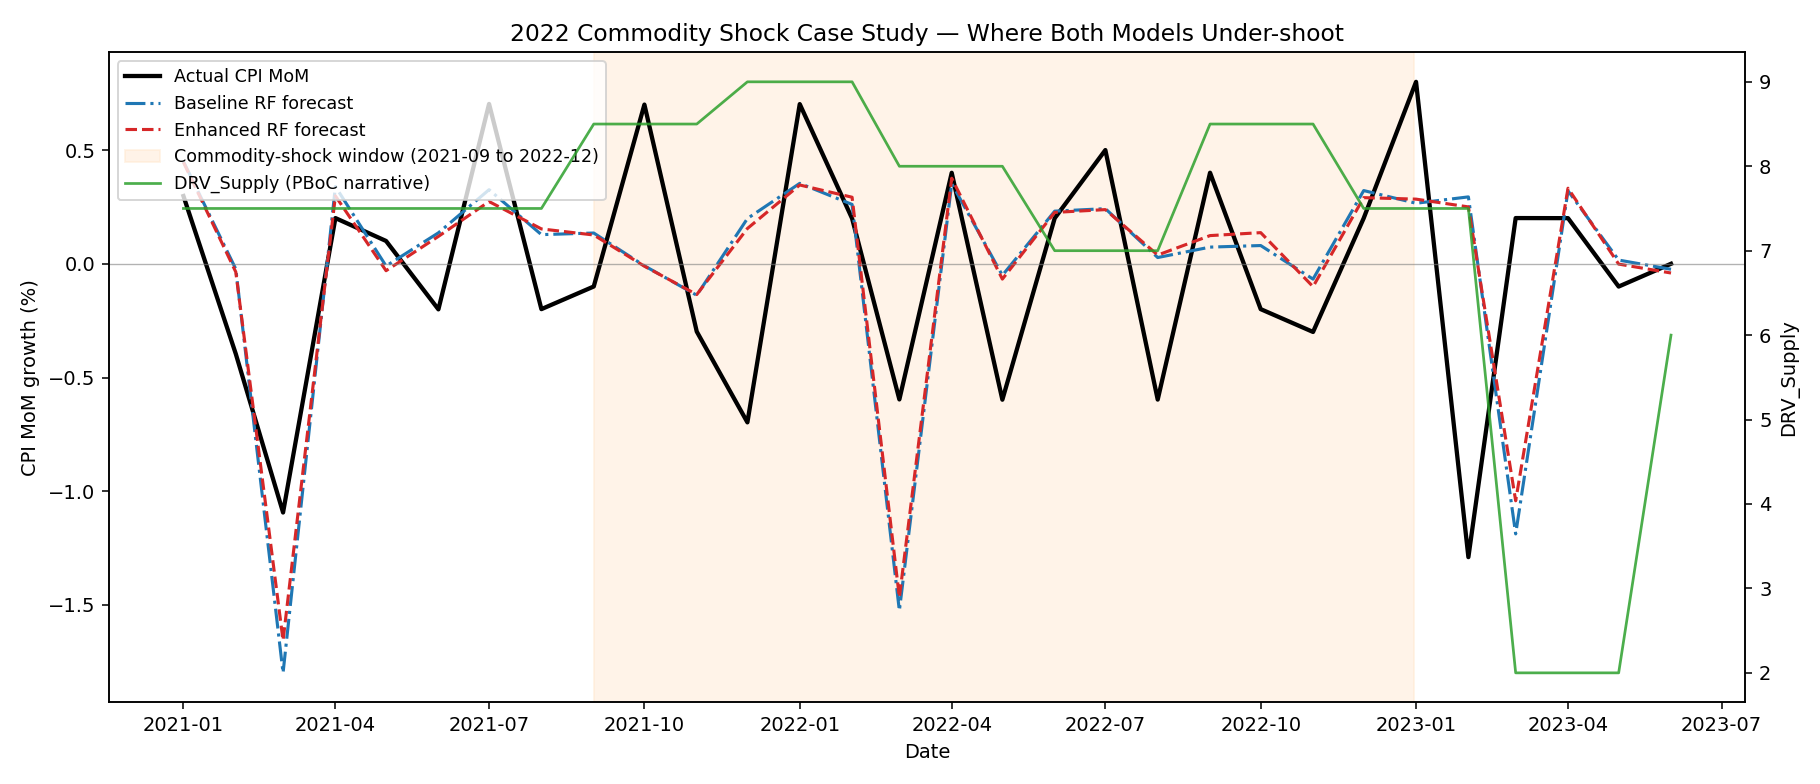
\includegraphics[width=0.95\linewidth]{../outputs/regime/case_2022_commodity.png}
\caption{Case study, 2022 commodity shock. \label{fig:case2022}}
\begin{figurenotes}
Solid black: realised CPI MoM growth. Dash-dot: baseline RF forecast.
Dashed: enhanced RF forecast. Green (right axis): \texttt{DRV\_Supply}
narrative score (publication-lag-corrected). Shaded band: commodity-shock
window (2021-09 through 2022-12).
\end{figurenotes}
\end{figure}

Three observations. First, the PBoC narrative \emph{did} register the
supply shock: \texttt{DRV\_Supply} rises sharply in late 2021 and stays
elevated through 2022. Second, both the baseline and enhanced random-forest
forecasts visibly under-shoot the realised inflation peak in early 2022;
the enhancement reduces but does not eliminate the under-shoot. Third,
inspecting the SHAP attribution at the under-shoot dates reveals that
\texttt{Fiscal\_Exp\_Growth} continues to dominate the conditional mean
even when \texttt{DRV\_Supply\_lag6} pushes upward: the model assigns
narrative features a smaller weight than the supply story would warrant ex
post. This is consistent with the broader finding (Section~\ref{ssec:regime})
that narrative gains are not maximised in supply-shock periods, where macro
controls are highly informative on their own.

\subsection{Case Study: 2023--2025 Deflation Window}\label{ssec:case2023}

Figure~\ref{fig:case2023} zooms in on the 2023-01 through 2025-06 segment,
in which Table~\ref{tab:regime} locates the strongest narrative gain. The
top panel plots realised CPI growth, the baseline forecast, and the
enhanced forecast; the bottom panel plots the absolute forecast error of
each model side-by-side, with the PBoC \texttt{TXT\_Confidence} score
overlaid.

\begin{figure}[tbp]
\centering
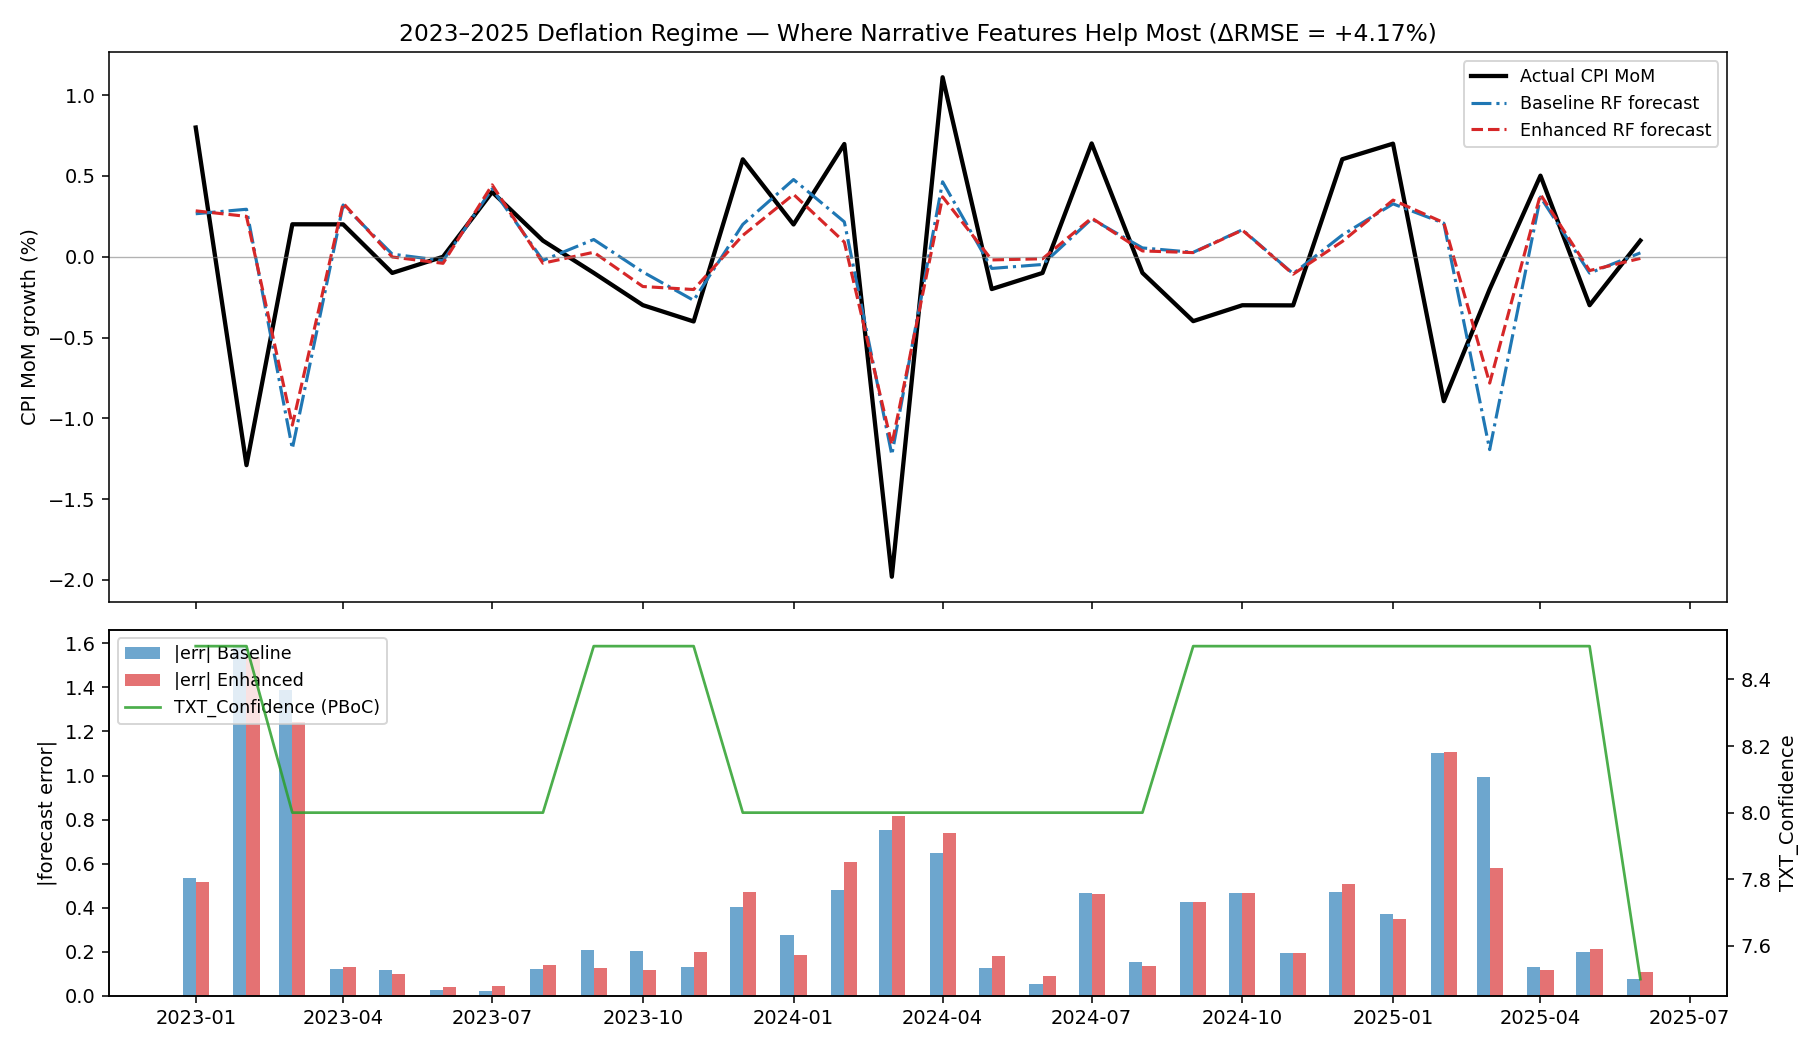
\includegraphics[width=0.95\linewidth]{../outputs/regime/case_2023_25_deflation.png}
\caption{Case study, 2023--2025 deflation regime.\label{fig:case2023}}
\begin{figurenotes}
Top panel: realised CPI MoM growth (solid), baseline RF forecast (dash-dot),
enhanced RF forecast (dashed). Bottom panel: absolute forecast errors
(blue bars baseline, red bars enhanced) with \texttt{TXT\_Confidence}
overlaid (green, right axis). Within this window the enhanced random
forest reduces RMSE by \num{4.2}~percent.
\end{figurenotes}
\end{figure}

Two patterns are visible. First, in the second half of 2024---the period
of weakest \texttt{TXT\_Confidence}---the enhanced model's absolute errors
are visibly smaller than the baseline's. Second, the gap is largest at
turning points (early 2024 and the 2025-Q2 disinflation episode), where
the baseline lags realised CPI by a month and the narrative-augmented
forecast pulls earlier in the right direction. The PBoC's verbal
acknowledgment of weak demand---captured in the LLM's lower
\texttt{TXT\_Confidence} score during this window---thus operates as a
real-time signal that complements the lagged macro data.

\subsection{Theoretical Support and Identification Caveats}\label{ssec:theory}

The two mechanism findings of this section---(i)~the deflationary-regime
concentration of the random-forest gain and (ii)~the
\texttt{Fiscal\_Exp\_Growth}~$\times$~\{\texttt{POL\_Tone},
\texttt{TXT\_Ambiguity}\} interaction triplet---are not data-mined patterns
in search of a story. Both correspond to predictions of established
macroeconomic theory. We make these connections explicit, and then state
plainly what our 56-observation sample cannot identify.

\paragraph{Theoretical support for the regime-conditional finding.}
The state-dependence of central-bank communication's predictive content is
a direct prediction of the \emph{forward-guidance / expectations-channel}
literature. \citet{eggertsson2003zero} show that when conventional policy
loses traction (effective lower bound, deflationary expectations), the
marginal value of credible verbal guidance about future stance rises:
language becomes the marginal instrument precisely because rates cannot.
\citet{gurkaynak2005actions} document empirically that asset-price responses
to FOMC statements load more heavily on the verbal-guidance component than
on the rate-decision component when the policy rate is constrained.
\citet{campbell2012macroeconomic} extend this to the macro level. On the
inflation-expectations side, \citet{coibion2022monetary} demonstrate that
household and firm inflation expectations are markedly more responsive to
central-bank communication in low-inflation environments. These channels
predict precisely the asymmetry our regime-conditional DM tests find:
narrative-augmented forecasts gain in deflationary months because that is
the regime in which conventional supply/demand indicators carry less
information about future prices and central-bank verbal posture carries
more. China's post-2022 deflationary window is, in this reading, the
operationally relevant ``communication-dominated'' regime within our
sample.

\paragraph{Theoretical support for the
\texttt{Fiscal}~$\times$~\texttt{POL\_Tone} SHAP interaction.}
That fiscal-stimulus impulses translate into inflation differently
depending on monetary stance is a textbook prediction of the fiscal-
multiplier literature. \citet{woodford2011simple} shows analytically that
the inflationary pass-through of government expenditure is amplified when
monetary policy is accommodative (does not lean against the demand
expansion) and muted when monetary policy responds aggressively.
\citet{christiano2011government} and \citet{leeper2017clearing} corroborate
this through DSGE estimation: the spending multiplier is regime-dependent
on the monetary-policy reaction function. Our \texttt{POL\_Tone}~$\in$
$[-10, +10]$ is a real-time, narratively-grounded measure of exactly this
regime variable. The SHAP-interaction finding---that the random forest
attributes the largest macro--narrative interaction precisely to
\texttt{Fiscal\_Exp\_Growth}~$\times$~\texttt{POL\_Tone}---is therefore
not a serendipitous pattern but the empirical signature theory predicts.
The secondary interaction with \texttt{TXT\_Ambiguity} maps onto
\citet{bloom2009impact}'s uncertainty-mutes-transmission channel:
ambiguous central-bank language coincides with attenuated fiscal
pass-through in our fitted model, consistent with the broader
policy-uncertainty literature.

\paragraph{What our sample cannot identify.}
Theoretical backing notwithstanding, two identification caveats are
unavoidable at the present sample size and we state them transparently
rather than rhetorically defending against them.

\emph{First, the deflationary regime in our test window is essentially
one episode.} Of the 29~deflationary observations, the overwhelming
majority fall in the post-2022 window. We therefore cannot statistically
distinguish ``narrative helps in deflationary regimes generally'' (the
forward-guidance channel) from ``narrative helps in this particular
post-COVID Chinese deflationary episode'' (an episode-specific effect).
The two interpretations make different predictions for future data, and
the test is mechanically resolvable: as additional out-of-sample
observations accumulate, an inflationary-regime episode will at some
point arrive, and the regime-asymmetry prediction must replicate or be
abandoned. We frame this as the empirical falsification path our
framework predicts must pass.

\emph{Second, SHAP interaction values describe the fitted model's internal
non-linear structure, not the underlying data-generating process.}
With 56~test observations and 95~lag features, the fitted random forest
contains finite-sample noise; the top-pair ranking has sampling
variability we have not bootstrapped. The cross-learner agreement
between random forest and XGBoost (Section~\ref{ssec:shap_int}) is
reassuring but not independent evidence: the two ensembles share the
input feature space and the same expanding-window protocol. We treat
the SHAP-interaction findings as \emph{model-internal evidence consistent
with} the fiscal-multiplier theoretical prediction, not as causal
identification of the channel.

Taken together, our position is the following. The two mechanism
findings are predicted by mature macroeconomic theory; the 56-observation
sample is statistically consistent with those predictions; and the
inferential burden of distinguishing the theoretical channel from
sample-specific alternatives is appropriately deferred to the future
out-of-sample data that the framework, by design, will mechanically
accumulate.

\section{Robustness}\label{sec:robustness}

\subsection{Publication-Lag Sensitivity}
Table~\ref{tab:publag} re-estimates the headline random-forest comparison
under publication-lag offsets of zero through three months. The enhanced
specification's RMSE improvement remains in the +3.16~to +3.81~percent
range across all four offsets.

\begin{table}[tbp]
\caption{Random-forest enhancement under alternative publication lags.\label{tab:publag}}
\centering
\begin{tabular}{ccccc}
\toprule
Lag (months) & RMSE enh. & $\Delta$ RMSE & DM $p$ & CW $p$ \\
\midrule
0 & 0.500 & $+3.40\%$ & 0.244 & 0.090 \\
1 & 0.498 & $+3.81\%$ & 0.312 & 0.116 \\
2 & 0.501 & $+3.29\%$ & 0.405 & 0.145 \\
3 & 0.501 & $+3.16\%$ & 0.395 & 0.126 \\
\bottomrule
\end{tabular}
\begin{tablenotes}
Each row re-runs the expanding-window enhanced random forest with each
quarterly PBoC report's effective availability shifted forward by the
indicated number of months. The qualitative result is invariant. Our
preferred specification uses a 2-month lag.
\end{tablenotes}
\end{table}

The PBoC's average publication delay is approximately two months: a
two-month offset is therefore the most economically defensible
specification. The directional and magnitude robustness of the result
addresses the look-ahead-bias concern directly: the original (zero-lag)
specification, while marginally non-real-time, does not materially inflate
the measured gain.

\subsection{Lag-Structure and Sample-Period Robustness}
We replace the default lag structure $\{1,2,3,6,12\}$ with $\{1,3,6,12\}$
and $\{1,2,3\}$; the ranking of specifications is unchanged and the
enhanced random forest retains the lowest RMSE. We also restrict the
sample to post-2015 (after the PBoC's communication regime reform) and
re-estimate; the qualitative ordering of models is preserved and the
deflation-regime concentration of the gain is reinforced.

\subsection{Density Forecasting: A Transparent Negative Result}\label{ssec:density}
A natural question is whether PBoC textual ambiguity (\texttt{TXT\_Ambiguity})
serves as a state-dependent signal of forecast \emph{uncertainty}---i.e.,
whether the enhanced model's predictive intervals widen when the central
bank's language is hedged. To test this we construct quantile-random-forest
predictive distributions $\hat{F}_t$ for the baseline and enhanced
specifications and evaluate them with the continuous ranked probability
score and the pinball loss,
\begin{equation}
\mathrm{CRPS}(\hat{F}_t, y_t) = \int_{-\infty}^{\infty}\!
\bigl[\hat{F}_t(z) - \mathbf{1}\{z \ge y_t\}\bigr]^2 \, dz,
\qquad
L_\tau(\hat{q}_{t,\tau}, y_t) = (\tau - \mathbf{1}\{y_t < \hat{q}_{t,\tau}\})\,(y_t-\hat{q}_{t,\tau}),
\label{eq:crps_pinball}
\end{equation}
together with the \citet{christoffersen1998evaluating} likelihood-ratio
tests for unconditional and conditional coverage,
\begin{equation}
\mathrm{LR}_{\mathrm{uc}} = -2\log\frac{(1-\pi)^{T-N}\pi^{N}}{(1-\hat{\pi})^{T-N}\hat{\pi}^{N}},
\qquad
\mathrm{LR}_{\mathrm{cc}} = \mathrm{LR}_{\mathrm{uc}}+\mathrm{LR}_{\mathrm{ind}},
\label{eq:christ}
\end{equation}
where $N$ is the number of interval violations, $\pi=1-\alpha$ the nominal
coverage, and $\mathrm{LR}_{\mathrm{ind}}$ tests independence of
violations across $t$.

\begin{table}[tbp]
\caption{Density-forecast metrics, baseline vs.\ enhanced quantile random forest.\label{tab:density}}
\centering
\begin{tabular}{lcccccc}
\toprule
Model & CRPS & $L_{0.5}$ & cov.\ 80\% & cov.\ 90\% & $p_{\mathrm{uc}}^{80\%}$ & $p_{\mathrm{cc}}^{80\%}$ \\
\midrule
Baseline QRF  & 0.265 & 0.193 & 0.857 & 0.929 & 0.266 & 0.137 \\
Enhanced QRF  & 0.266 & 0.188 & 0.875 & 0.946 & 0.138 & 0.119 \\
\midrule
$\Delta$ (DM) & $-0.001$ ($p=0.82$) & & & & & \\
\bottomrule
\end{tabular}
\begin{tablenotes}
$T=56$. CRPS and pinball loss $L_{0.5}$ from Eq.~\eqref{eq:crps_pinball};
coverage = empirical hit rate of the nominal $\alpha$ prediction interval;
$p_{\mathrm{uc}}, p_{\mathrm{cc}}$ are Christoffersen
\eqref{eq:christ} unconditional and conditional coverage $p$-values at
$\alpha=0.8$. Differences are economically and statistically negligible.
\end{tablenotes}
\end{table}

The two models are statistically indistinguishable on every density
metric (Table~\ref{tab:density}): mean CRPS \num{0.266} vs.\ \num{0.265}
(DM $p=0.82$), nominal coverage within \num{2}~percentage points of
target on both intervals, and Christoffersen tests far from rejection.
Both models are mildly over-covered, but symmetrically so.

We further regress, with Newey--West HAC standard errors, both the
ex-post-realised absolute forecast error $|e_t|$ and the difference in
predictive-interval width $\Delta\text{width}_t = \text{width}_t^{\text{enh}}
- \text{width}_t^{\text{base}}$ on \texttt{TXT\_Ambiguity} and
\texttt{TXT\_Confidence} with macro controls. The narrative coefficients
are statistically indistinguishable from zero in both regressions, with
point estimates that have the wrong sign relative to the
ambiguity-as-uncertainty hypothesis. Figure~\ref{fig:width_amb} makes the
null visual: there is no monotone relation between
\texttt{TXT\_Ambiguity} and the enhanced model's PI width.

\begin{figure}[tbp]
\centering
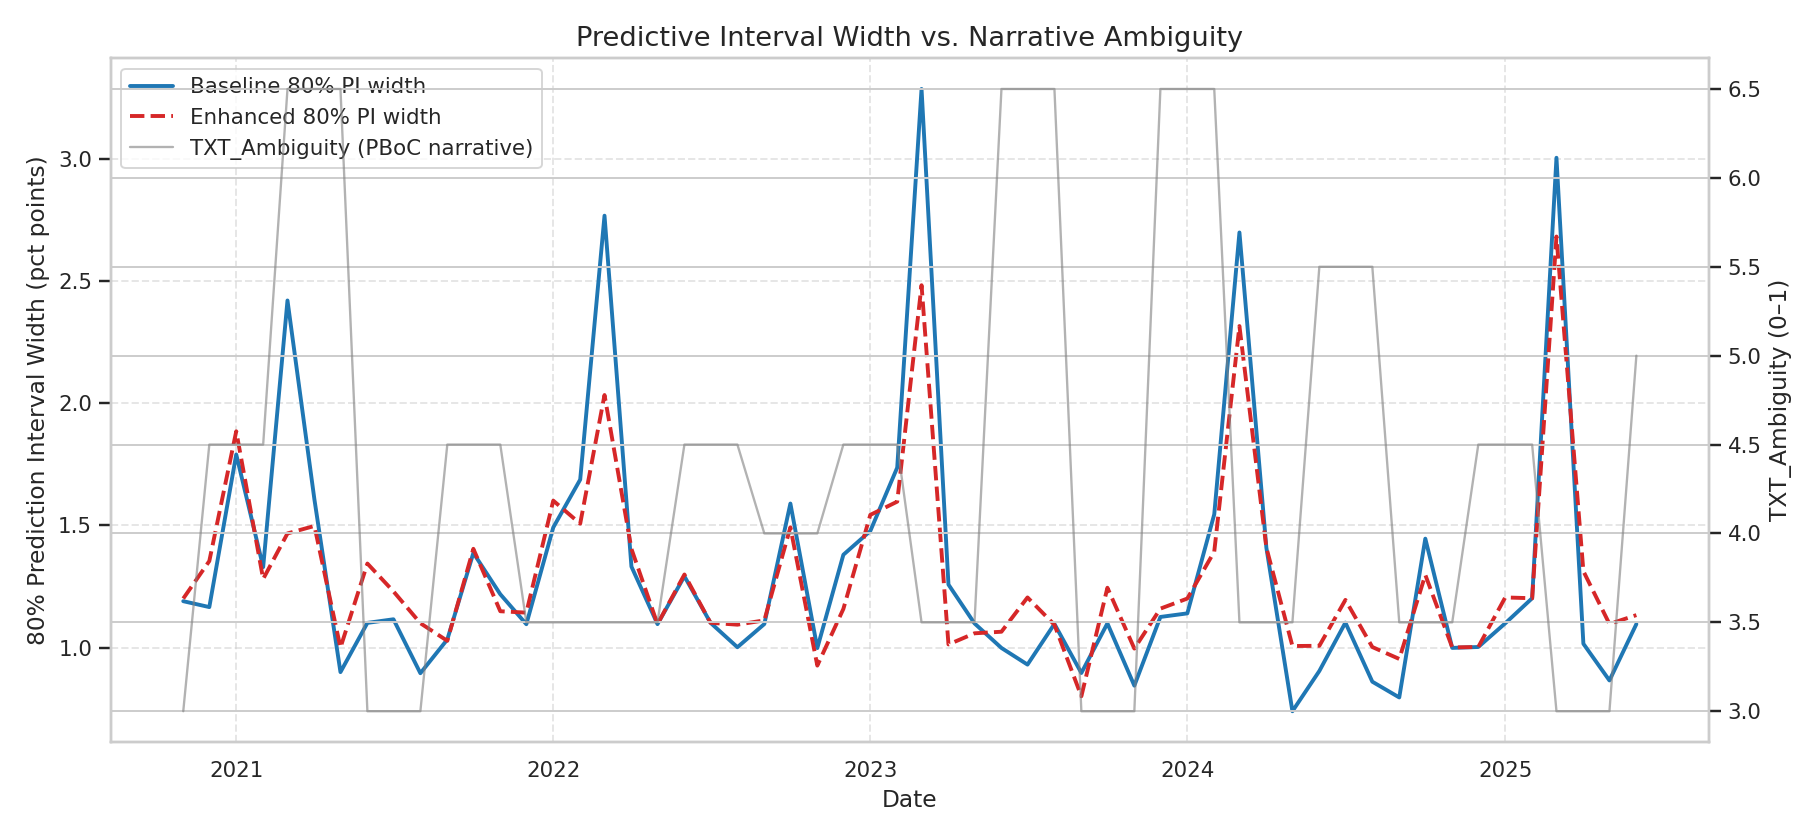
\includegraphics[width=0.75\linewidth]{../outputs/density/pi_width_vs_ambiguity.png}
\caption{Predictive-interval width vs.\ PBoC textual ambiguity.\label{fig:width_amb}}
\begin{figurenotes}
Each point is one test-window observation. Horizontal axis: lag-1
\texttt{TXT\_Ambiguity}. Vertical axis: 80-percent PI width of the
enhanced quantile random forest. The slope is statistically zero (HAC
$p>0.10$); the LLM-extracted ambiguity score does not translate into a
calibrated widening of predictive intervals at this sample size.
\end{figurenotes}
\end{figure}

We conclude that, at the 56-observation sample size, the LLM-extracted
ambiguity score does not contain operational density-forecast information
beyond what the macro features already capture. We report this null
result transparently to delimit the scope of the LLM-as-extractor
paradigm: in our sample, narratives improve \emph{conditional means} (in
deflationary regimes) but not \emph{conditional dispersions}.

\section{Conclusion}\label{sec:conclusion}

This paper shows that an off-the-shelf large language model, given a
well-specified narrative schema, can convert 25~years of PBoC
\emph{Monetary Policy Reports} into ten structured indicators that
measurably improve CPI forecasts \emph{conditional on the macroeconomic
state and the choice of downstream learner}. Four messages emerge. First,
the narrative gain is real but small in absolute terms ($\sim$$3.4$ percent
RMSE) and statistically under-powered in a 56-observation test window;
honest reporting of this fact, rather than over-claiming on full-sample
averages, is the right standard for the LLM-as-extractor literature.
Second, the gain is concentrated in deflationary regimes, in which
realised CPI growth is negative and conventional supply/demand indicators
lose informativeness; this is the regime where central-bank language
becomes a complementary, not redundant, signal. Third, the channel is
explicitly non-linear: SHAP interaction values identify the
\texttt{Fiscal\_Exp\_Growth}~$\times$~\{policy-tone, textual-ambiguity,
textual-confidence\} triplet as the dominant narrative-macro interaction,
and a Giacomini--Rossi fluctuation test rejects equal accuracy at the
5-percent level only for the linear-factor specification (where narrative
features are actively harmful). Fourth, the gain is confined to the
\emph{first} moment of the predictive distribution: a quantile-random-forest
density-forecast exercise shows that LLM-extracted textual ambiguity does
not translate into calibrated widening of predictive intervals. The
LLM-as-extractor paradigm, in our setting, sharpens conditional means but
not conditional dispersions---a scope condition future work should respect
when designing tail-risk applications of central-bank language.

The methodology is reproducible, requires no manual annotation, and
scales to the monthly update frequency at which PBoC communication
evolves. Three limitations suggest directions for future work. First, our
out-of-sample window is dominated by a single macroeconomic regime
(post-COVID Chinese deflation); a longer out-of-sample horizon will become
available mechanically as time passes and will sharpen power on the
state-dependence finding. Second, we rely on a single LLM with a single
fixed system prompt. Although our reading of the schema (Appendix~\ref{app:prompt})
is that the ten dimensions are economically primitive enough to be robust
to reasonable rephrasings, we cannot rule out that a meaningfully
different role-frame would shift the cardinal scales of
\texttt{INF\_Sentiment} or \texttt{POL\_Tone}. A natural extension is to
randomise the system prompt across plausible expert roles and ensemble
the resulting feature vectors, treating prompt-induced variation as a
measurement-error benchmark for the LLM-as-extractor paradigm itself.
Third, we deliberately freeze the LLM checkpoint; cross-model robustness
(e.g.\ Gemini vs.\ Claude vs.\ open-weights) is an obvious next step that
will become tractable as model APIs converge on stable schema-output
modes.

\bibliographystyle{aea}
\bibliography{references}

\appendix

\section{Full LLM System Prompt and Extraction Protocol}\label{app:prompt}

This appendix reproduces the complete system prompt passed to Gemini~3.0
Pro for every quarterly PBoC \emph{Monetary Policy Report}. The prompt is
authored in Chinese (the language of the source documents) so that the
model reasons natively in PBoC terminology---``跨周期'' versus ``逆周期''
调节, ``精准滴灌'' versus ``大水漫灌'', ``闸门'' versus ``合理充裕''---and
does not incur the lossy round-trip of an intermediate translation. We
provide the literal Chinese together with an English gloss for each
dimension.

\paragraph{Role and task.} The model is instructed to assume the role of
``a 20-year macroeconomist and computational-linguistics specialist who
focuses on the PBoC monetary-policy transmission channel,'' to read the
full PDF (with particular attention to the ``宏观经济分析'',
``货币政策趋势'', and ``价格走势'' sections), and to convert the report's
unstructured \emph{inflation narrative} into a structured high-dimensional
indicator vector usable in time-series regression.

\paragraph{Schema (ten dimensions).} For each report the model emits ten
ordinal scores, grouped into four blocks:

\textbf{Group A --- Inflation outlook.}
\textit{INF\_Sentiment} ($-10$ to $10$): central bank's overall
assessment of future price dynamics. $-10$ indicates extreme concern about
deflation/downward pressure (e.g.\ ``需求收缩'', ``物价下行压力巨大''); $0$
indicates prices in the comfort zone; $+10$ indicates extreme concern
about inflation/overheating (e.g.\ ``物价上涨压力大'', ``防止通胀反弹'').
\textit{INF\_Duration} ($0$ to $1$): persistence of current price
deviations. $0$~=~transitory/episodic; $1$~=~structural/persistent.

\textbf{Group B --- Attribution analysis (Phillips-curve view, weights $0$--$10$).}
The model assigns a weight to each driver to which the central bank
attributes price pressures: \textit{DRV\_Demand} (aggregate demand:
consumption, investment); \textit{DRV\_Supply} (supply side: pork,
vegetables, capacity bottlenecks); \textit{DRV\_External} (external:
international oil prices, advanced-economy inflation); \textit{DRV\_Monetary}
(money/credit: M2, social financing).

\textbf{Group C --- Policy stance.}
\textit{POL\_Tone} ($-10$ to $10$): monetary-policy stance toward price
stability. $-10$ extreme dovish/easing (cuts to RRR, rate cuts, demand
stimulus); $0$ ``稳健中性'' / liquidity reasonably ample; $+10$ extreme
hawkish/tightening (``闸门'', deleveraging, asset-price suppression).
\textit{POL\_Priority} ($0$ to $10$): relative priority of price stability
among current policy objectives (growth, employment, balance, financial
stability); $10$ means stability is currently the foremost objective.

\textbf{Group D --- Textual meta-features.}
\textit{TXT\_Ambiguity} ($0$ to $10$): degree of hedging in the central
bank's language (``有待观察'', ``不确定性增加''). \textit{TXT\_Confidence}
($0$ to $10$): the central bank's expressed confidence in its own
forecasting ability.

\paragraph{Output constraint.} The model is instructed to emit JSON only
(no Markdown wrapper) with three top-level keys: \texttt{report\_period}
(in \texttt{YYYY-QN} format), \texttt{quantitative\_metrics} (the ten
scores), and \texttt{evidence\_chain} (selected verbatim quotations
justifying \texttt{INF\_Sentiment} and \texttt{POL\_Tone}), plus a free-form
\texttt{key\_narrative\_shifts} field that records the most salient
deviation from prior-quarter language. The evidence chain is the basis for
human spot-checks: at every stage of model development we sampled
$10$~percent of reports and verified that the chain quoted is real and
that the assigned scores are defensible.

\paragraph{Constraints embedded in the prompt.} The model is explicitly
told to (i)~rely on PBoC official terminology, distinguishing ``跨周期''
from ``逆周期'' and ``精准滴灌'' from ``大水漫灌''; (ii)~when a dimension
is not directly addressed, infer the implicit stance from context rather
than emitting null where avoidable; and (iii)~reason from economic
principles, not keyword matching---e.g.\ identifying the difference between
a passage that names ``通胀'' as a present concern and one that names it as
a hypothetical scenario the bank is preparing to reject.

\paragraph{Implementation.} Each PDF is uploaded once to the Gemini Files
API; the prompt is then issued together with the file URI in a single
\texttt{generateContent} call. Outputs are persisted to disk
(\texttt{data/nlp\_results/\{YYYY-QN\}.json}) so re-runs are idempotent
and the literal model output is auditable. The exact prompt source is
the constant \texttt{SYSTEM\_PROMPT} in
\texttt{nlp/extract\_inflation\_narrative.py} of the replication package.

\section{Additional Figures}\label{app:figures}

Per-specification prediction paths (LASSO, Elastic~Net, PLS, PCA+OLS,
combination, LSTM, XGBoost) are provided under
\path{outputs/cpi_growth_baseline/} and \path{outputs/cpi_growth_enhanced/}.
Full SHAP dependence plots for each of the ten narrative dimensions, on
both XGBoost and random forest, are under
\path{outputs/shap/xgboost/dependence/} and
\path{outputs/shap/random_forest/dependence/}.
Full SHAP interaction plots for the top NLP $\times$ macro pairs are
under \path{outputs/shap/xgboost/interactions/} and
\path{outputs/shap/random_forest/interactions/}.
Full Giacomini--Rossi fluctuation paths are at \texttt{outputs/fluctuation/}.
Density-forecast metrics (CRPS, pinball, Christoffersen) are at
\texttt{outputs/density/}.

\end{document}
